\documentclass{article}
\usepackage[utf8]{inputenc}
\topmargin=0cm
\oddsidemargin=0cm
\textheight=22.0cm
\textwidth=18cm
\parindent=0cm
\parskip=0.15cm
\topskip=0truecm
\raggedbottom
\setcounter{secnumdepth}{4}
\setcounter{tocdepth}{2}
\abovedisplayskip=3mm
\belowdisplayskip=3mm
\abovedisplayshortskip=0mm
\belowdisplayshortskip=2mm
\normalbaselineskip=10pt
\normalbaselines
\usepackage{pdfpages}
\usepackage{xcolor}
\usepackage{graphicx}
\usepackage[T1]{fontenc}
\usepackage{textcomp}
\usepackage{amsthm}
\usepackage{tcolorbox}
\usepackage{amsmath, amssymb}
\usepackage{enumitem}
\usepackage{transparent}
\usepackage{tabulary}
\usepackage[affil-it]{authblk}
\usepackage{minted}
\usepackage{changepage}
\usepackage{hyperref}
\usepackage{adjustbox}
\usepackage[a4paper, total={6.5in, 9in}]{geometry}
\graphicspath{ {./imgs/} }
\setminted[MYSQL]{ 
    breaklines=true,
    numbersep=5pt,
    frame=single,
    numbersep=5pt,
    xleftmargin=0.1cm,
    xrightmargin=0.1cm,
    style = native,
    bgcolor = LightGray
    }
\setminted[php]{ 
    breaklines=true,
    numbersep=5pt,
    frame=single,
    numbersep=5pt,
    xleftmargin=0.1cm,
    xrightmargin=0.1cm,
    bgcolor = LightGray,
    style = monokai
    }

\date{April 2021}

\begin{document}
               \includepdf[pages=-]{EoO.pdf}

                \vspace*{3in}
                \centerline{\bf\Large COMP 353, Winter 2021}
                \centerline{\bf\Large Team Project - Final Project}

                \vspace*{0.5in}
                \centerline{\bf\Large Team 4 (ydc353\_4)}

                \vspace*{0.5in}
                \centerline{\today}

                \vspace*{0.5in}
                \begin{table}[htbp]
                    \begin{center}
                        \begin{tabular}{|r | c| c|}
                            \hline
                            Name & ID Number & GitHub Username \\
                            \hline\
                            Antoine Assal & 40022745 & @As.Antoine  \\
                            \hline
                            Benjamin Lofo Follo & 40008156 & @lamungu \\ 
                            \hline
                            Rami Bou Abboud & 40043011 & @Mr Robot \\
                            \hline
                            Ribelle El Ayoubi & 29276726  & @Belle-coder\\
                            \hline
                        \end{tabular}
                    \end{center}
                \end{table}
                \newpage
\tableofcontents
\listoffigures

\newpage
\listoftables
\newpage


\section{Assumptions}
Show your reasonable Assumptions made in the proposed database design.
\begin{itemize}
    \item Every user in our database is a Person. However, for a Person to exist they must be a Patient or a Health Care worker.
    \item A Healthcare worker can be a patient, not mutually exclusive.
    \item Auto-incrementing identifiers for our entities avoids user input which eliminates the possibility of errors of having multiple instance of an entity with the same ID.
    \item Our database system will be used to cover Canada and it's region/cities.
    \item Our data focuses on Quebec.
    \item Regions, GroupZones, and Recommendation do not need a delete call in CRUD.
\end{itemize}

\section{E/R diagram}
E/R diagram to represent the conceptual database design for the application.

\begin{figure}[H]
    \centering
    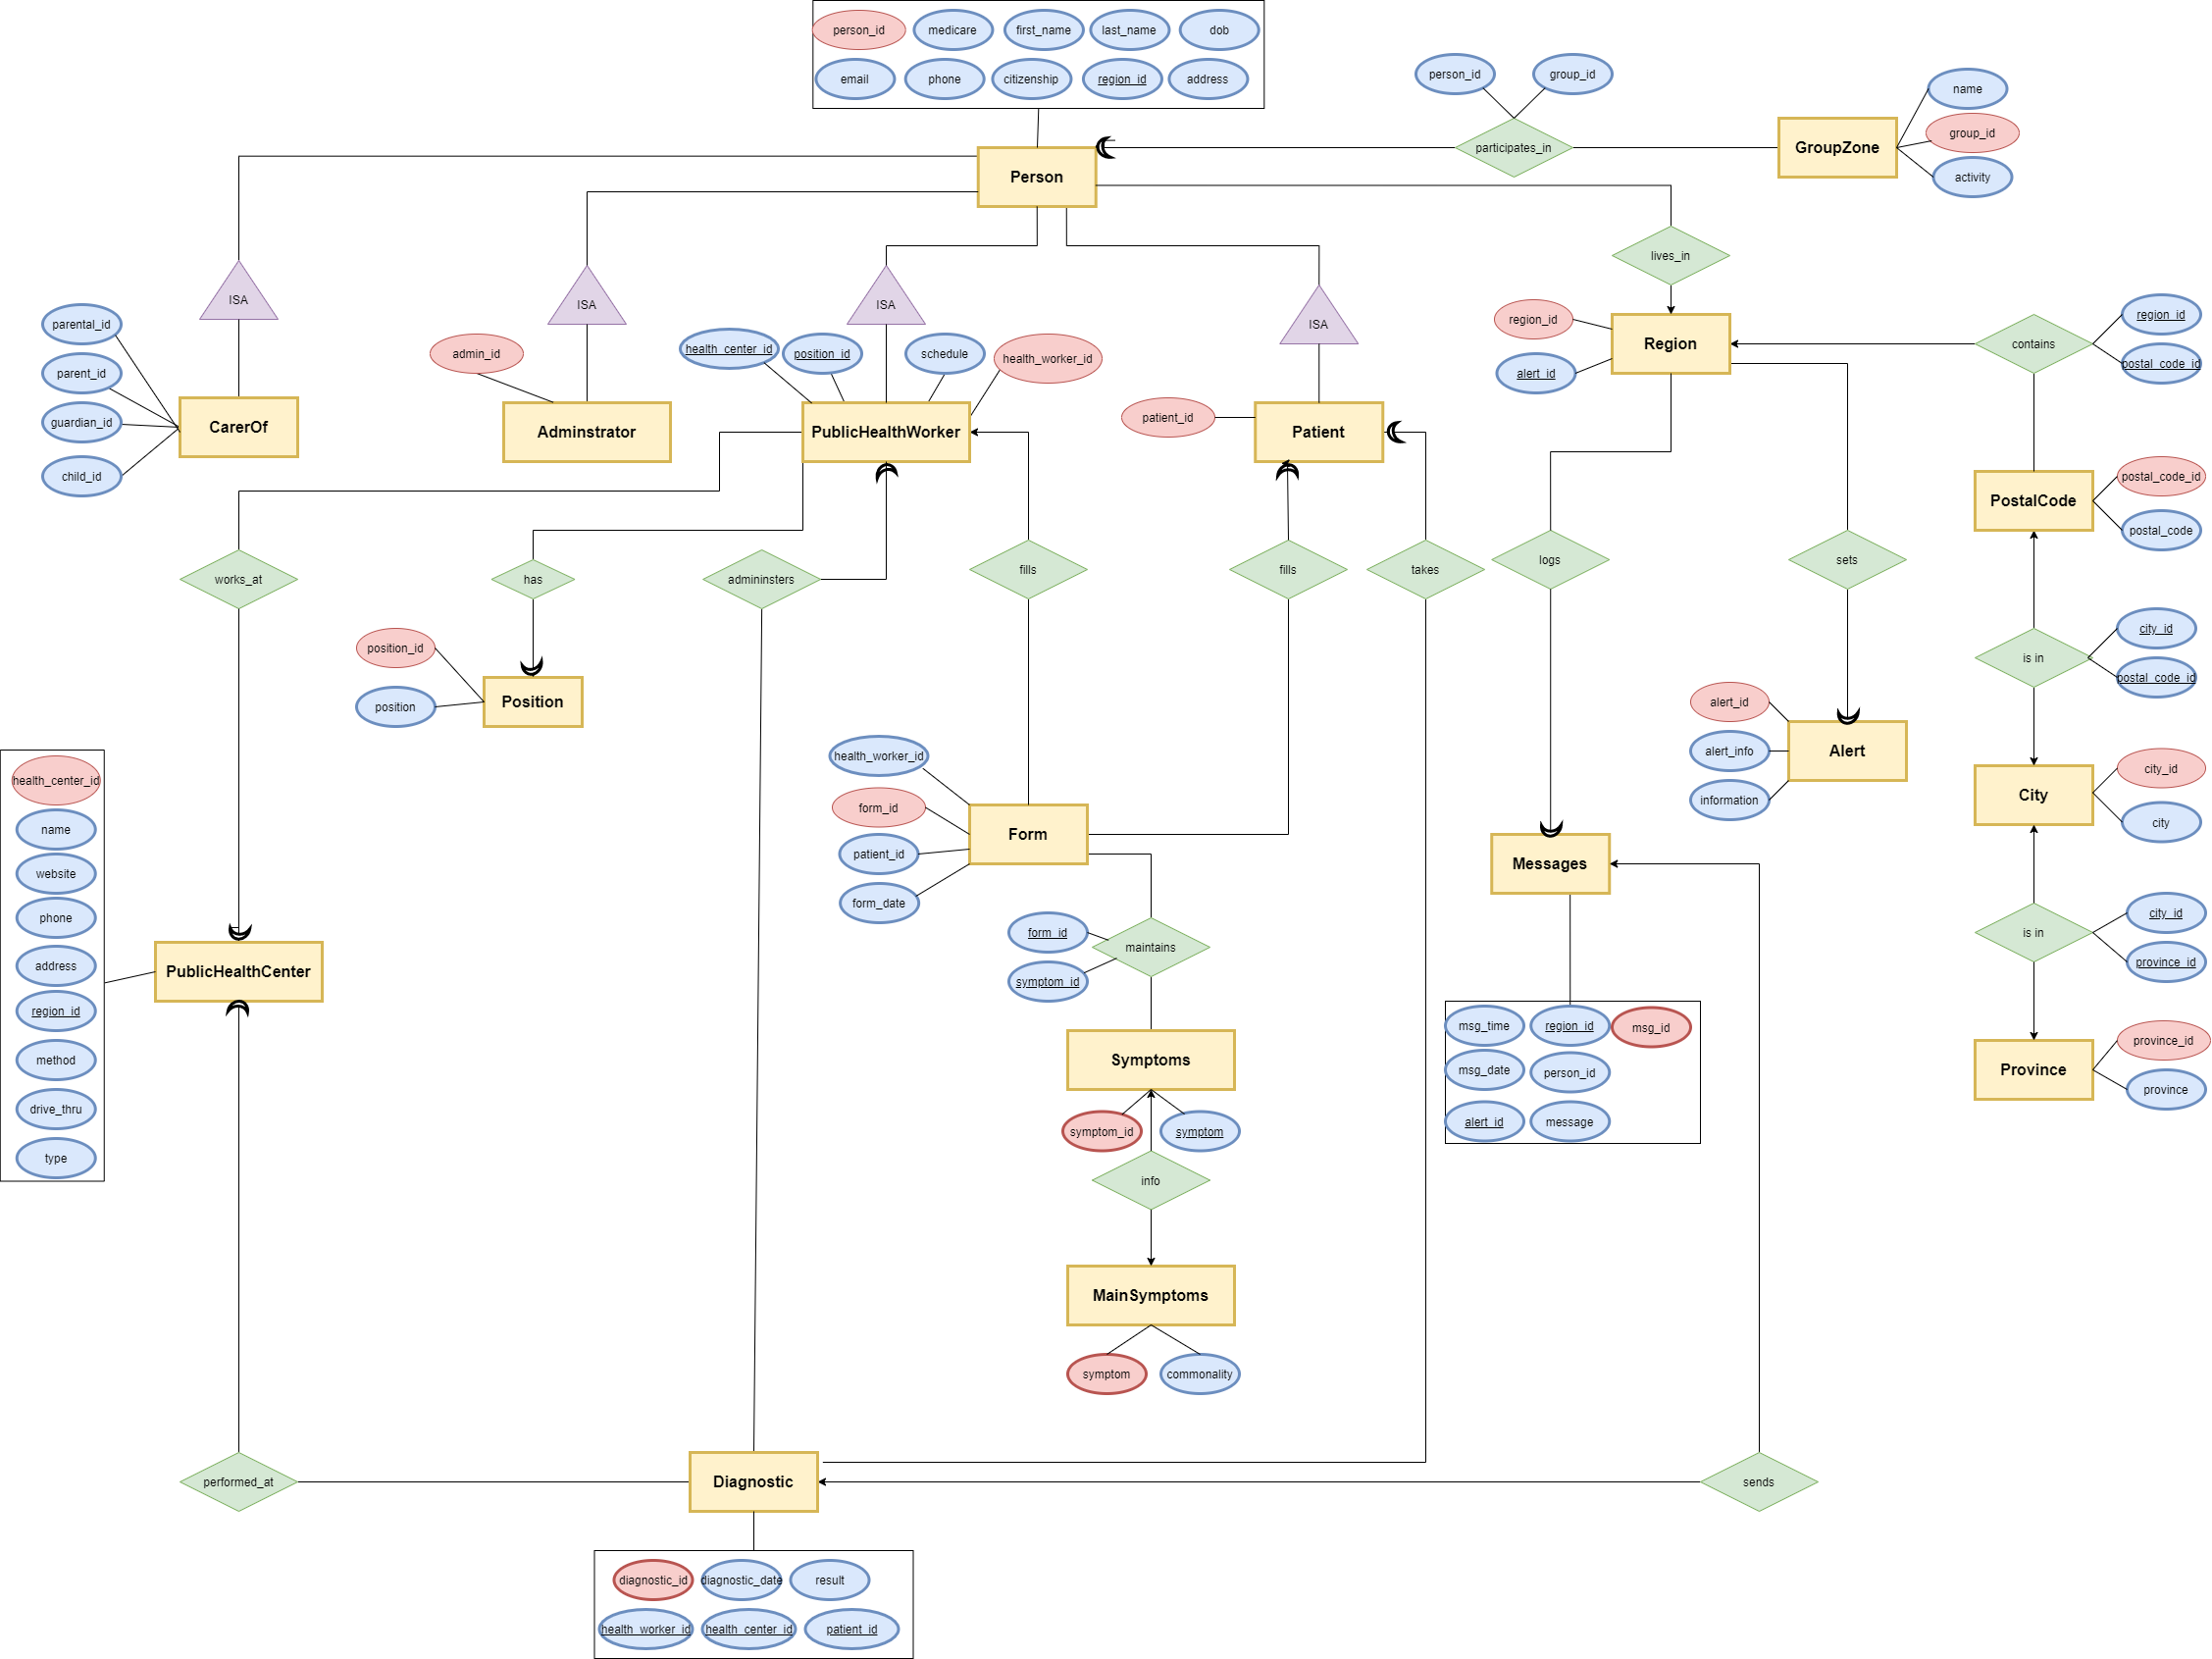
\includegraphics[scale=0.22]{imgs/ERD.PNG}
    \caption{E/R diagram}
\end{figure}

\subsection{Constraints captured by the diagram}
\begin{itemize}
    \item Multiplicity of relationships (pointed arrow)
    \item Inheritance (Triangle)
    \item Referential Integrity (Curved arrow)
    \item Primary keys (red bubble)
    \item Foreign keys (underlined attribute)
\end{itemize}
\subsection{Constraints not captured by the diagram}
One of the limitations we came across when using this notation is having referential integrity and multiplicity pointing to the same entity and we had cases where referential integrity and multiplicity of relationships conflicted.
\begin{itemize}
    \item We prioritized showing the referential integrity constraint. 
    \item We did not show referential integrity on the ERD when it comes to inherited entity sets.
    \item The diagram does not capture data types.
    \item The diagram does not capture Nullable attributes.
    \item The diagram does not show functional dependencies.
\end{itemize} 
\subsection{A different notation}
\begin{figure}[H]
    \centering
    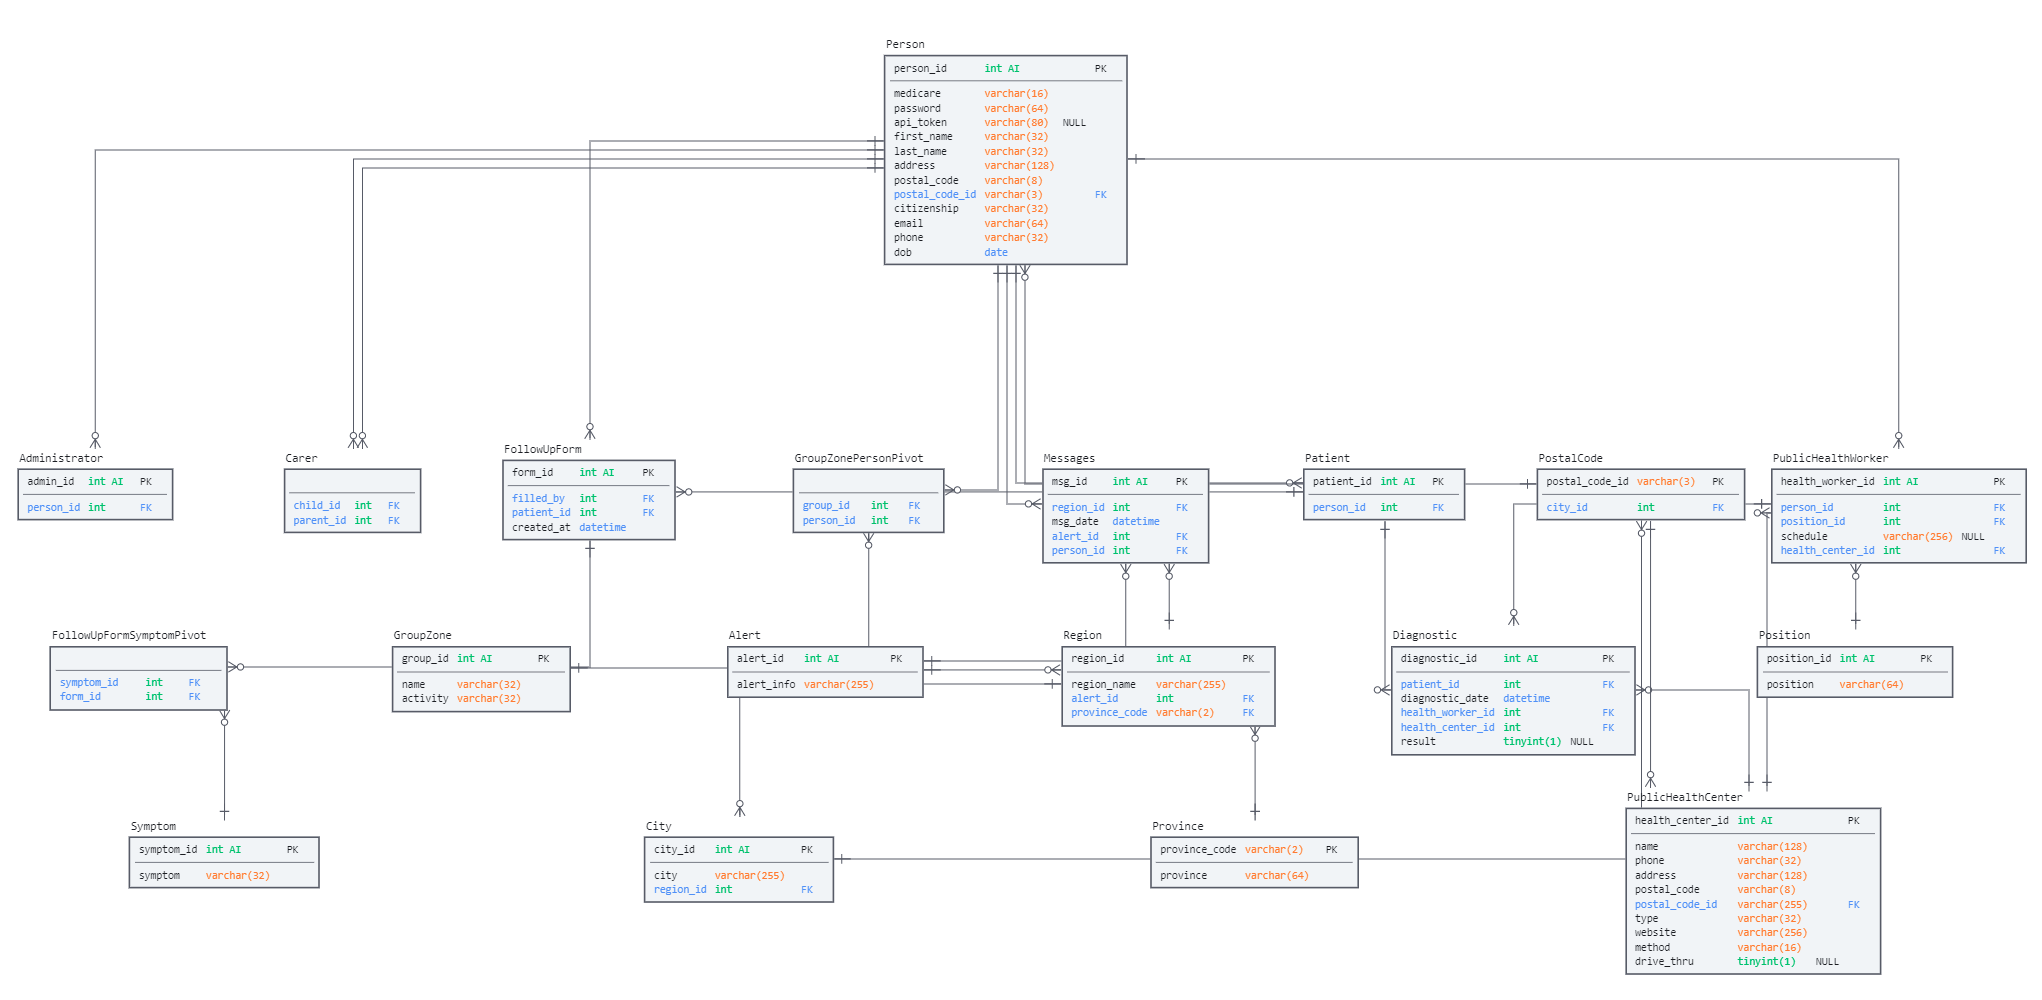
\includegraphics[scale=0.34]{imgs/nOtAnErD.png}
    \caption{A diagram that captures some more constraints (NOT AN ERD)}
\end{figure}
\newpage

\section{Relational Database Schema}
Convert your E/R diagram into a relational database schema. Make refinements to
the DB schema if necessary. Identify various integrity constraints such as primary
keys, foreign keys, functional dependencies, and referential constraints. Make sure
that your database schema is at least in 3NF.

\subsection{Relational Model from Warm-up Project}
This is the Relational schema we came up with for the warm-up project. Underline represents a primary key and \# represents a foreign key.
\begin{itemize}
    \item Person (\underline{person\_id}, medicare, first\_name, last\_name, address, city, postal\_code, province, citizenship, email, phone, dob)
    \item Parental (\underline{parental\_id}, \#person\_id, parent\_1\_id, parent\_2\_id, guardian\_id, child\_id)
    \item PublicHealthWorker (\underline{health\_worker\_id}, position, schedule,  \#health\_center\_id, \#person\_id)
    \item PublicHealthCenter (\underline{health\_center\_id}, phone, name, address, city, province, postal\_code, type, website)
    \item Diagnostic (\underline{diagnostic\_id}, diagnostic\_date, result, \#health\_worker\_id, \#health\_center\_id, \#person\_id)
    \item Patient (\underline{patient\_id}, \#person\_id)
    \item GroupZone (\underline{group\_id}, activity, name)
    \item GroupZonePersonPivot (\underline{group\_id}, \underline{person\_id})
\end{itemize}

\subsection{Relational Model with Updated Information}
For this project, we read the instructions carefully and started building on top of our schema to have a new one that includes all the new required information for our system.
\begin{itemize}
    \item Person (\underline{person\_id}, medicare, first\_name, last\_name, address, city, postal\_code, province, citizenship, email, phone, dob, password, api\_token)
    \item Patient (\underline{patient\_id}, \#person\_id, symptoms, symptoms\_history)
    \item Carer (\underline{parental\_id}, \#person\_id, parent\_1\_id, parent\_2\_id, guardian\_id, child\_id)
    \item PublicHealthWorker (\underline{health\_worker\_id}, position, schedule,\#health\_center\_id, \#person\_id)
    \item PublicHealthCenter (\underline{health\_center\_id}, phone, name, address, city, province, postal\_code, type, website, drive\_thru)
    \item Diagnostic (\underline{diagnostic\_id}, diagnostic\_date, result,\#health\_worker\_id, \#health\_center\_id, \#patient\_id)
    \item FollowupForm (\underline{form\_id}, \#health\_worker\_id, \#patient\_id)
    \item GroupZone (\underline{group\_id}, activity, name)
    \item Region (\underline{region\_id}, region\_name, city, postal\_code, province)
    \item Alert (\underline{alert\_id}, alert\_name, alert\_level, alert\_region, alert\_status, alert\_date, alert\_time, current\_alert, past\_alert, message, \#person\_id, recommendation)
    \end{itemize}

\subsection{Model's Normal Form}
It is safe to say that our model is at least in \textbf{1NF} for all the relations since all attributes are atomic and cannot contain more than one value. The only exception is symptoms \& symptoms\_history, which will be normalized later in this document.
\subsubsection{Person}
For the Person Relation we have the following non-trivial dependencies:\\
\begin{minipage}{\textwidth}
\begin{itemize}
    \item \{person\_id\} $\rightarrow$ first\_name
    \item \{person\_id\} $\rightarrow$ last\_name
    \item \{person\_id\} $\rightarrow$ medicare
    \item \{person\_id\} $\rightarrow$ password
    \item \{person\_id\} $\rightarrow$ address
    \item \{person\_id\} $\rightarrow$ postal\_code
    \item \{person\_id\} $\rightarrow$ citizenship
    \item \{person\_id\} $\rightarrow$ email
    \item \{person\_id\} $\rightarrow$ phone
    \item \{person\_id\} $\rightarrow$ dob
    \item \{person\_id\} $\rightarrow$ api\_token
    \item \{address\} $\not \rightarrow$ first\_name
    \item \{email\} $\not \rightarrow$ person\_id
\end{itemize}
\end{minipage}
person\_id cannot be determined, is not on the RHS of any of the FDs, making it a super-key and the only candidate key.

\begin{tcolorbox}
\textbf{So our $F$ is}:
\begin{multline}
$ F = \{ person\_id \rightarrow first\_name,last\_name, medicare, password,\\
address, postal\_code, citizenship, email, phone, dob, api\_token \} $
\end{multline}
\begin{multline}
$person\_id^+ = \{person\_id, first\_name,last\_name, medicare, password,\\
address,postal\_code, citizenship, email, phone, dob, api\_token \} $
\end{multline}

Key = $person\_id$\\
This relation is \textbf{in 2NF}.\\
This relation is \textbf{in 3NF}.\\
This relation is \textbf{in BCNF}.
\end{tcolorbox}
\newpage

\subsubsection{Carer}

For the Carer Relation we have the following non-trivial dependencies:\\

\begin{minipage}{\textwidth}
\begin{itemize}
    \item \{person\_id\} $\rightarrow$ child\_id
    \item \{person\_id\} $\rightarrow$ parent\_1\_id
    \item \{person\_id\} $\rightarrow$ parent\_2\_id
    \item \{person\_id\} $\rightarrow$ guardian\_id
    \item \{parent\_1\_id\} $\rightarrow$ child\_id
    \item \{parent\_2\_id\} $\rightarrow$ child\_id
    \item \{parent\_1\_id, parent\_2\_id\} $\rightarrow$ child\_id
    \item \{parent\_1\_id, parent\_2\_id, guardian\_id\} $\rightarrow$ child\_id
\end{itemize}
\end{minipage}

\begin{tcolorbox}
    \textbf{So our $F$ is}:
\begin{multline}
$F = \{ \{ person\_id \rightarrow child\_id, parent\_1\_id, parent\_2\_id, guardian\_id \}, \\
\{parent\_1\_id \rightarrow child\_id\} , \{parent\_2\_id \rightarrow child\_id\} , \\
\{parent\_1\_id, parent\_2\_id, guardian\_id \rightarrow child\_id \} \} $
\end{multline}
This relation is \textbf{not in 2NF} because we have partial dependencies, \\
For example $person\_id \rightarrow parent\_1\_id$ and we can split it into more tables. 
\end{tcolorbox}

\subsubsection{PublicHealthWorker}
For the PublicHealthWorker Relation we have the following non-trivial dependencies:\\
\\
\begin{minipage}{\textwidth}
\begin{itemize}
    \item \{health\_worker\_id\} $\rightarrow$ position
    \item\{health\_worker\_id\}  $\rightarrow$ schedule
    \item \{health\_worker\_id\}  $\rightarrow$ health\_center\_id
    \item \{health\_worker\_id\}  $\rightarrow$ person\_id
    \item \{health\_center\_id\}  $\not \rightarrow$ health\_worker\_id\\
\end{itemize}
\end{minipage}
\\
health\_worker\_id cannot be determined, is not on the RHS of any of the FDs, making it a super-key and the only candidate key.
\begin{tcolorbox}
    \textbf{So our $F$ is}:
$F = \{health\_worker\_id \rightarrow position, schedule, health\_center\_id, person\_id\}$\\
\\
$health\_worker\_id^+ = \{health\_worker\_id, person\_id, position, schedule, health\_center\_id \}$\\
\\
Key = $health\_worker\_id$\\
This relation is \textbf{in 2NF}.\\
This relation is \textbf{in 3NF}.\\
This relation is \textbf{in BCNF}.
\end{tcolorbox}

\subsubsection{PublicHealthCenter}
For the PublicHealthCenter Relation we have the following non-trivial dependencies:\\
\\
\begin{minipage}{\textwidth}
\begin{itemize}
    \item \{health\_center\_id\} $\rightarrow$ phone
    \item\{health\_center\_id\}  $\rightarrow$ name
    \item \{health\_center\_id\}  $\rightarrow$ address
    \item \{health\_center\_id\}  $\rightarrow$ city
    \item \{health\_center\_id\}  $\rightarrow$ province
    \item \{health\_center\_id\}  $\rightarrow$ postal\_code
    \item \{health\_center\_id\}  $\rightarrow$ type
    \item \{health\_center\_id\}  $\rightarrow$ website
    \item \{health\_center\_id\}  $\rightarrow$ drive\_thru
    \item \{postal\_code\}  $\rightarrow$ city
    \item \{postal\_code\}  $\rightarrow$ province
    \item \{city\}  $\rightarrow$ province
\end{itemize}
\end{minipage}

\begin{tcolorbox}
    \textbf{So our $F$ is}:
\begin{multline}
$F = \{ \{health\_center\_id \rightarrow phone, name, address, city, province, postal\_code, type, website,\\ 
drive\_thru\} , \{postal\_code \rightarrow city, province\}, \{city \rightarrow province\} \}$
\end{multline}
Key = $health\_worker\_id$ \\
This relation is \textbf{in 2NF}.\\
$postal\_code \rightarrow city, province$ \textbf{violates 3NF rules.}\\
It is non-trivial, LHS is not a superkey and RHS contains a non-key attribute.\\
This relation is \textbf{not in 3NF}.\\
This relation is \textbf{not in BCNF}.
\end{tcolorbox}
\newpage
\subsubsection{Diagnostic}
For the Diagnostic Relation we have the following non-trivial dependencies:\\
\\
\begin{minipage}{\textwidth}
\begin{itemize}
    \item  \{diagnostic\_id\}   $\rightarrow$ diagnostic\_date
    \item\ \{diagnostic\_id\}   $\rightarrow$ result
    \item  \{diagnostic\_id\}   $\rightarrow$ health\_worker\_id
    \item  \{diagnostic\_id\}   $\rightarrow$ health\_center\_id\
    \item  \{diagnostic\_id\}   $\rightarrow$ patient\_id
    \item  \{patient\_id\,health\_worker\_id\} $\not \rightarrow$ diagnostic\_id
    \item  \{patient\_id\,health\_worker\_id\} $\not \rightarrow$ result
\end{itemize}
\end{minipage}

\begin{tcolorbox}
\textbf{So our $F$ is}:
$F = \{diagnostic\_id \rightarrow diagnostic\_date, result, health\_worker\_id, health\_center\_id\}$\\
Key = $diagnostic\_id$\\
diagnostic\_id cannot be determined, is not on the RHS of any of the FDs, making it a super-key and the only candidate key.\\
This relation is \textbf{in 2NF}.\\
This relation is \textbf{in 3NF}.\\
This relation is \textbf{in BCNF}.
\end{tcolorbox}

\subsubsection{FollowUpForm}
For the FollowUpForm Relation we have the following non-trivial dependencies:\\
\\
\begin{minipage}{\textwidth}
\begin{itemize}
    \item  \{form\_id\}   $\rightarrow$ health\_worker\_id
    \item  \{form\_id\}   $\rightarrow$ patient\_id
\end{itemize}
\end{minipage}
form\_id cannot be determined, is not on the RHS of any of the FDs, making it a super-key and the only candidate key.
\begin{tcolorbox}
    \textbf{So our $F$ is}:
$F = \{form\_id \rightarrow health\_worker\_id, patient\_id\}$\\
\\
$form\_id^+ = \{form\_id, health\_worker\_id, patient\_id\}$\\
\\
Key = $form\_id$\\
This relation is \textbf{in 2NF}.\\
This relation is \textbf{in 3NF}.\\
This relation is \textbf{in BCNF}.
\end{tcolorbox}
\newpage
\subsubsection{GroupZone}
For the Groupzone Relation we have the following non-trivial dependencies:\\
\\
\begin{minipage}{\textwidth}
\begin{itemize}
    \item  \{group\_id\}   $\rightarrow$ activity
    \item  \{group\_id\}   $\rightarrow$ name
\end{itemize}
\end{minipage}
group\_id cannot be determined, is not on the RHS of any of the FDs, making it a super-key and the only candidate key.
\begin{tcolorbox}
    \textbf{So our $F$ is}:
$F = \{group\_id \rightarrow activity, name \}$\\
\\
$group\_id^+ = \{group\_id, activity, name\}$\\
\\
Key = $group\_id$\\
This relation is \textbf{in 2NF}.\\
This relation is \textbf{in 3NF}.\\
This relation is \textbf{in BCNF}.
\end{tcolorbox}
\subsubsection{Region}
For the Region Relation we have the following non-trivial dependencies:\\
\\
\begin{minipage}{\textwidth}
\begin{itemize}
    \item  \{region\_id\}   $\rightarrow$ region\_name
    \item  \{region\_id\}   $\rightarrow$ city
    \item  \{region\_id\}   $\rightarrow$ postal\_code
    \item  \{region\_id\}   $\rightarrow$ province
    \item \{postal\_code\}  $\rightarrow$ city
    \item \{postal\_code\}  $\rightarrow$ province
    \item \{city\}  $\rightarrow$ province

\end{itemize}
\end{minipage}
\begin{tcolorbox}
    \textbf{So our $F$ is}:
\begin{multline}
$F = \{ \{region\_id \rightarrow region\_name, city, postal\_code, province\}, \\
\{postal\_code \rightarrow city, province\}, \{city \rightarrow province\} \}$
\end{multline*}
\\
This relation is \textbf{in 2NF}.\\
$postal\_code \rightarrow city, province$ \textbf{violates 3NF rules.}\\
It is non-trivial, LHS is not a superkey and RHS contains a non-key attribute.\\
This relation is \textbf{not in 3NF}.\\
This relation is \textbf{not in BCNF}.
\end{tcolorbox}

\newpage
\subsubsection{Alert}
For the Alert Relation we have the following non-trivial dependencies:\\
\\
\begin{minipage}{\textwidth}
\begin{itemize}
    \item \{alert\_id\}   $\rightarrow$ alert\_name
    \item \{alert\_id\}   $\rightarrow$ alert\_level
    \item \{alert\_id\}   $\rightarrow$ alert\_region
    \item \{alert\_id\}   $\rightarrow$ alert\_status
    \item \{alert\_id\}   $\rightarrow$ alert\_date
    \item \{alert\_id\}   $\rightarrow$ alert\_time
    \item \{alert\_id\}   $\rightarrow$ current\_alert
    \item \{alert\_id\}   $\rightarrow$ past\_alert
    \item \{alert\_id\}   $\rightarrow$ message
    \item \{alert\_id\}   $\rightarrow$ person\_id
    \item \{alert\_id\}   $\rightarrow$ recommendation
    \item \{alert\_region\}   $\rightarrow$ alert\_status
    \item \{alert\_region\}   $\rightarrow$ alert\_level
    \item \{alert\_region\}   $\rightarrow$ message
    \item \{message\}   $\rightarrow$ recommendation
    \item \{person\_id} $\rightarrow$ message
\end{itemize}
\end{minipage}

\begin{tcolorbox}
    \textbf{So our $F$ is}:
\begin{multline}
$F = \{ \{alert\_id \rightarrow alert\_name, alert\_level, alert\_region, alert\_status, alert\_date, \\ alert\_time, current\_alert, past\_alert, message, person\_id, recommendation\} , \\
\{alert\_region \rightarrow alert\_status, alert\_level, message\}, \\
\{message \rightarrow recommendation\}, \{person\_id \rightarrow message \}\}$
\end{multline}
Key = $alert\_id$\\
This relation is \textbf{in 2NF}.\\
$alert\_region \rightarrow alert\_status, alert\_level, message$ \textbf{violates 3NF rules.}\\
It is non-trivial, LHS is not a superkey and RHS contains a non-key attribute.\\
This relation is \textbf{not in 3NF}.\\
This relation is \textbf{not in BCNF}.
\end{tcolorbox}
\newpage
\subsection{Few Relation instances}
\subsubsection{Person}
api\_token and password are randomly generated numbers or hashed strings. Shortened them for the report.
\begin{table}[H]
\centering
\begin{adjustbox}{width=1.2\textwidth,center=\textwidth}
\begin{tabular}{|l|l|l|l|l|l|l|l|l|l|l|l|l|l|} 
        \hline
        person\_id & medicare & first\_name & last\_name & address & city & postal\_code & province & citizenship & email & phone & dob & password & api\_token \\
        \hline 
4 & GBUJ46611976 & Anne & Paquette & 6577 Sébastien Plains & Sainte-Catherine & G3N 0O9 & QC & KN & bstpierre@lapierre.com & 1-882-823-4013, & 1977-02-08 & KxsFhruN & gwh0XS \\    
16 & EEKJ96363064 & Marc & Gauthier & 756 Tessier Prairie & Montreal & H1H 7D2 & QC & TF & brigitte92@lambert.com & 470-997-1115, & 1990-06-29 & zd9Znke & xO3TUV\\        
        \hline
\end{tabular}
\end{adjustbox}
\caption{Un-normalized person relation instance}
\end{table}
\begin{table}[H]
\centering
\begin{adjustbox}{width=1.2\textwidth,center=\textwidth}
\begin{tabular}{|l|l|l|l|l|l|l|l|l|l|l|l|l|l|} 
        \hline
        person\_id & medicare & first\_name & last\_name & address & postal\_code & postal\_code\_id & citizenship & email & phone & dob & password & api\_token \\
        \hline 
4 & GBUJ46611976 & Anne & Paquette & 6577 Sébastien Plains & G3N 0O9 & G3N & KN & bstpierre@lapierre.com & 1-882-823-4013, & 1977-02-08 & KxsFhruN & gwh0XS \\    
16 & EEKJ96363064 & Marc & Gauthier & 756 Tessier Prairie & H1H 7D2 & H1H & TF & brigitte92@lambert.com & 470-997-1115, & 1990-06-29 & zd9Znke & xO3TUV\\        
        \hline
\end{tabular}
\end{adjustbox}
\caption{Normalized person relation instance}
\end{table}


\subsubsection{Patient}
\begin{table}[H]
\centering
\begin{adjustbox}{width=0.5\textwidth,center=\textwidth}
\begin{tabular}{|l|l|l|l|} 
        \hline
        patient\_id & person\_id & symptoms & symptoms\_history \\ 
        \hline
        1 & 11 & cough,fever & cough,fever,loss of taste\\
        6 & 16 & NULL & NULL\\
        \hline
\end{tabular}
\end{adjustbox}
\caption{Un-normalized patient relation instance}
\end{table}

\begin{table}[H]
\centering
\begin{adjustbox}{width=0.2\textwidth,center=\textwidth}
\begin{tabular}{|l|l|} 
        \hline
        patient\_id & person\_id \\ 
        \hline
        1 & 11 \\
        6 & 16 \\
        \hline
\end{tabular}
\end{adjustbox}
\caption{Normalized patient relation instance}
\end{table}



\subsubsection{Carer}
\begin{table}[H]
\centering
\begin{adjustbox}{width=0.6\textwidth,center=\textwidth}
\begin{tabular}{|l|l|l|l|l|l|} 
        \hline
        parental\_id & person\_id & parent\_1\_id & parent\_2\_id & guardian\_id & child\_id\\ 
        \hline
        1 & 4 & 5 & 7 & NULL & 4\\
        2 & 9 & NULL & NULL & 11 & 9\\
        \hline
\end{tabular}
\end{adjustbox}
\caption{Un-normalized carer relation instance}
\end{table}

\begin{table}[H]
\centering
\begin{adjustbox}{width=0.2\textwidth,center=\textwidth}
\begin{tabular}{|l|l|} 
        \hline
        child\_id & parent\_id \\ 
        \hline
        4 & 5 \\
        4 & 7 \\
        9 & 11 \\
        \hline
\end{tabular}
\end{adjustbox}
\caption{Normalized carer relation instance}
\end{table}

\newpage
\subsubsection{PublicHealthWorker}
\begin{table}[ht]
\centering
\begin{adjustbox}{width=1\textwidth,center=\textwidth}
\begin{tabular}{|l|l|l|l|l|} 
        \hline
        health\_worker\_id & person\_id & position & schedule & health\_center\_id\\ 
        \hline
        1 & 18 & Doctor & Mon: 19:00-03:00, Tue: 07:00-15:00 & 4\\
        2 & 12 & Nurse & Thu: 04:00-12:00, Fri: 17:00-01:00, Sat: 09:00-17:00 & 5\\
        \hline
\end{tabular}
\end{adjustbox}
\caption{Un-normalized PublicHealthWorker relation instance}
\end{table}

\begin{table}[ht]
\centering
\begin{adjustbox}{width=1\textwidth,center=\textwidth}
\begin{tabular}{|l|l|l|l|l|} 
        \hline
        health\_worker\_id & person\_id & position & schedule & health\_center\_id\\ 
        \hline
        1 & 18 & 1 & Mon: 19:00-03:00, Tue: 07:00-15:00 & 4\\
        2 & 12 & 2 & Thu: 04:00-12:00, Fri: 17:00-01:00, Sat: 09:00-17:00 & 5\\
        \hline
\end{tabular}
\end{adjustbox}
\caption{Normalized PublicHealthWorker relation instance}
\end{table}

\subsubsection{Position}
\begin{table}[H]
\centering
\begin{adjustbox}{width=0.2\textwidth,center=\textwidth}
\begin{tabular}{|l|l|} 
        \hline
        position\_id & position \\ 
        \hline
        1 & Doctor \\
        2 & Nurse \\
        3 & Intern \\
        \hline
\end{tabular}
\end{adjustbox}
\caption{Normalized Position relation instance}
\end{table}


\subsubsection{PublicHealthCenter}
\begin{table}[H]
\centering
\begin{adjustbox}{width=1.2\textwidth,center=\textwidth}
\begin{tabular}{|l|l|l|l|l|l|l|l|l|l|} 
        \hline
        health\_center\_id & phone & name & address & city & province & postal\_code & type & website & drive\_thru\\ 
        \hline
        4 & (828) 624-4739 & Boucher-Jacques & 1717 Boucher Well & Saint-Laurent & QC & H4T 4V7 & Hospital & www.simard.biz & 0\\
        5 & +1.903.423.4085 & Guay Ltd & T448 Girard Lane Suite 134 & Laval & QC & H7N 5N3 & Clinic & www.gangon.info & 1\\
        \hline
\end{tabular}
\end{adjustbox}
\caption{Un-normalized PublicHealthCenter relation instance}
\end{table}

\begin{table}[H]
\centering
\begin{adjustbox}{width=1.2\textwidth,center=\textwidth}
\begin{tabular}{|l|l|l|l|l|l|l|l|l|l|} 
        \hline
        health\_center\_id & phone & name & address & postal\_code\_id& postal\_code & type & website & method & drive\_thru\\ 
        \hline
        4 & (828) 624-4739 & Boucher-Jacques & 1717 Boucher Well & H4T & H4T 4V7 & Hospital & www.simard.biz & appointment & 0\\
        5 & +1.903.423.4085 & Guay Ltd & T448 Girard Lane Suite 134 & H7N & H7N 5N3 & Clinic & www.gangon.info & walk-in & 1\\
        \hline
\end{tabular}
\end{adjustbox}
\caption{Normalized PublicHealthCenter relation instance}
\end{table}

\subsubsection{PostalCode}
\begin{table}[H]
\centering
\begin{adjustbox}{width=0.25\textwidth,center=\textwidth}
\begin{tabular}{|l|l|} 
        \hline
        postal\_code\_id & city\_id \\ 
        \hline
        V1R & 229 \\
        V2K & 244 \\
        V7A & 304 \\
        \hline
\end{tabular}
\end{adjustbox}
\caption{Normalized PostalCode relation instance}
\end{table}

\subsubsection{City}
\begin{table}[H]
\centering
\begin{adjustbox}{width=0.35\textwidth,center=\textwidth}
\begin{tabular}{|l|l|l|} 
        \hline
        city\_id & city & region\_id \\ 
        \hline
        229 & Trail & 95 \\
        244 & Prince George North & 101 \\
        304 & Richmond South  & 126\\
        \hline
\end{tabular}
\end{adjustbox}
\caption{Normalized City relation instance}
\end{table}

\subsubsection{Region}
\begin{table}[H]
\centering
\begin{adjustbox}{width=0.45\textwidth,center=\textwidth}
\begin{tabular}{|l|l|l|l|l|} 
        \hline
        region\_id & region\_name & city & postal\_code & province \\ 
        \hline
        95 & Trail & Trail & V1R & British Columbia \\
        101 & Prince George & Prince George North & V2K & British Columbia \\
        126 & Richmond & Richmond South & V7A & British Columbia\\
        \hline
\end{tabular}
\end{adjustbox}
\caption{Un-normalized Region relation instance}
\end{table}

\begin{table}[H]
\centering
\begin{adjustbox}{width=0.45\textwidth,center=\textwidth}
\begin{tabular}{|l|l|l|l|l|} 
        \hline
        region\_id & region\_name & alert\_id & province\_id \\ 
        \hline
        95 & Trail & 1 & BC \\
        101 & Prince George North & 1 & BC\\
        126 & Richmond South  & 1 & BC\\
        \hline
\end{tabular}
\end{adjustbox}
\caption{Normalized Region relation instance}
\end{table}


\subsubsection{Province}
\begin{table}[H]
\centering
\begin{adjustbox}{width=0.35\textwidth,center=\textwidth}
\begin{tabular}{|l|l|l|l|l|} 
        \hline
        province\_id & province \\ 
        \hline
        BC & British Columbia\\
        SK & Saskatchewan\\
        QC & Quebec\\
        \hline
\end{tabular}
\end{adjustbox}
\caption{Normalized Province relation instance}
\end{table}

\newpage
% *********** Section 4 % *********** %
\section{Normalization}
Simple definitions for deriving normal forms :
\begin{itemize}
    \item 1NF : The key (remove repeating groups)
    \item 2NF : The whole key (remove partial dependence)
    \item 3NF : And nothing but the key (remove indirect dependence)
\end{itemize}

\subsection{Functional Dependency}
Already analysed each relation's $FD$s in section 3.3
\subsection{Normalization Steps}
\subsubsection{2NF}
\begin{tcolorbox}
    \textbf{Second Normal Form 2NF}: achieved by first making sure the table is in first normal form, and then removing attributes that only partially depend on the key by creating new tables. So the steps are :
    \begin{itemize}
        \item The Database is in \textbf{1NF}
        \item For every non-trivial dependency $X\rightarrow A$ either
        \begin{itemize}
            \item $X$ is not a proper subset of any candidate key OR
            \item $A$ is a key attribute
        \end{itemize}
    \end{itemize}
     \textbf{Key attribute}: An attribute that is part of some candidate key.\\
     \textbf{Super key}: A combination of fields that can uniquely determine a row \\
    \textbf{Candidate key}: A Super key that is also minimal. Meaning that :
     \begin{itemize}
         \item All candidate keys are super keys. 
         \item If we remove any field it's not a super key anymore.
     \end{itemize}
\end{tcolorbox}
We have already shown that the Carer relation is not in 2NF and needs to be normalized.

\paragraph{Carer}
We have redundant attributes, and we can simplify it by getting rid of \\
$parent\_1\_id$, $parent\_2\_id$ and $guardian\_id$.\\
Now our Carer relation is \\
Carer (\#parent\_id, \#child\_id)\\
This relation is now \textbf{in 2NF}.\\
This relation is now \textbf{in 3NF}.\\
This relation is now \textbf{in BCNF}.

\subsubsection{3NF}
\begin{tcolorbox}
    \textbf{Third Normal Form 3NF}: achieved by first making sure the table is in second normal form, and making sure that there are no non-key attributes that are transitively dependent on any candidate key.So the steps are :
    \begin{itemize}
        \item The Relation is in \textbf{2NF}
        \item If it's in 2NF and it's non-key attributes are fully and directly dependent on the key, then it is also in \textbf{3NF}
        \item For every non-trivial dependency $X\rightarrow A$ either
        \begin{itemize}
            \item $X$ is a superkey or 
            \item $A$ is a key attribute
        \end{itemize}
    \end{itemize}
\end{tcolorbox}
We have already shown that the \textbf{PublicHealthCenter, Region} and \textbf{Alert} relations are not in 3NF and need to be normalized.
\paragraph{PublicHealthCenter}
\begin{itemize}
    \item The set of candidate keys for this relation is $\{health\_center\_id\}$.
    \item Merge the $FDs$ we provided in 3.3.4, combining the same LHS whose RHS are non-key attributes.
    \item $R_1 = health\_center\_id \rightarrow drive\_thru, website, type, postal\_code, address, name, phone$
    \item $R_2 = postal\_code \rightarrow city$
    \item $R_3 = city \rightarrow province$
    \item Now $R_1$ is in 3NF.
    \item $R_2$ \& $R_3$ violate 3NF since their LHS is not a superkey and RHS is a set of non-key attributes.
    \item We will make a new table for them:
    \item Province(\underline{province\_code}, province)
    \item City(\underline{city\_id}, city, \#region\_id)
    \item Now PublicHealthCenter(\underline{health\_center\_id}, phone, name, address, postal\_code,\#postal\_code\_id, type, website, drive\_thru)
\end{itemize}
This relation is \textbf{in 2NF}.\\
This relation is now \textbf{in 3NF}.\\
This relation is now \textbf{in BCNF}.
\paragraph{Region} 
\begin{itemize}
    \item Same process is used as PublicHealthCenter so we get:
    \item Province(\underline{province\_code}, province)
    \item City(\underline{city\_id}, city, \#region\_id)
    \item Region(\underline{region\_id}, region\_name, \#province\_code)
    \end{itemize}
This relation is \textbf{in 2NF}.\\
This relation is now \textbf{in 3NF}.\\
This relation is now \textbf{in BCNF}.
\subsubsection{BCNF}

\begin{tcolorbox}
    \textbf{Boyce-Codd Normal Form BCNF}: achieved by first making sure the table is in third normal form. So the steps are :
    \begin{itemize}
        \item The Relation is in \textbf{3NF}
        \item For every non-trivial dependency $X\rightarrow A$, $A$ is a superkey.
    \end{itemize}
\end{tcolorbox}

We have already showed that Person, PublicHealthWorker, PublicHealthCenter, Region, Diagnostic, FollowUpForm, GroupZone and Alert are all in \textbf{BCNF}.

\subsection{Final Normalized Model}
\begin{tcolorbox}
\textbf{This is our final normalized model of the system.} All
\begin{itemize}
    \item Person (\underline{person\_id}, medicare, first\_name, last\_name, address, postal\_code, \#postal\_code\_id, citizenship, email, phone, dob, password, api\_token)
    \item Patient (\underline{patient\_id}, \# person\_id)
    \item Carer (\#child\_id, \#parent\_id)
    \item Administrator(\underline{admin\_id}, \#person\_id
    \item PublicHealthWorker (\underline{health\_worker\_id}, \#position\_id, schedule,\#health\_center\_id, \#person\_id)
    \item PublicHealthCenter (\underline{health\_center\_id}, phone, name, address, postal\_code,\#postal\_code\_id, type, website, method, drive\_thru)
    \item Position (\underline{position\_id}, position)
    \item Diagnostic (\underline{diagnostic\_id}, diagnostic\_date, result,\#health\_worker\_id, \#health\_center\_id, \#patient\_id)
    \item FollowUpForm (\underline{form\_id}, \#filled\_by, \#patient\_id, created\_at)
    \item Symptom (\underline{symptom\_id}, symptom)
    \item FollowUpFormSymptomPivot(\#symptom\_id, form\_id)
    \item GroupZone (\underline{group\_id}, activity, name)
    \item GroupZonePersonPivot(\#group\_id, \#person\_id)
    \item Region (\underline{region\_id}, region\_name, \#alert\_id, \#province\_code)
    \item Alert (\underline{alert\_id}, alert\_info)
    \item Province(\underline{province\_code}, province)
    \item City(\underline{city\_id}, city, \#region\_id)
    \item PostalCode (\underline{postal\_code\_id}, \#city\_id)
    \item Recommendation (\underline{recommendation\_id}, recommendation)
    \item Messages (\underline{msg\_id},\#region\_id, msg\_date, \#alert\_id, \#person\_id)
    \end{itemize}
    \end{tcolorbox}
\newpage
\subsection{Analysis of 3NF and BCNF}
The database design has been normalised to comply with the normalisation rules up to Third Normal Form (3NF). There are no redundant data that are related, as we split them all into their own tables. These tables are each identified by their own ID (primary key). 
If some data is related to more than one record, there has been a separate table created for it. Such tables are connected through foreign keys or, in some \textbf{special cases}, a separate pivot table has been created. Additionally, there are no values in the tables that do not depend on the key and we did not need any composite keys\\
Below is a list of all the \textbf{special cases} that required pivot tables.
\begin{itemize}
    \item \textbf{FollowupFormSymptomPivot}: Used to map a specific record of followup form to multiple records of symptom.
    \item \textbf{GroupZonePersonPivot}: Used to map a specific record of person form to multiple records of person.
\end{itemize}
We have shown in earlier sections that every relation has its own single super key and candidate key. 
There are no attributes that depend on non-key attributes in our tables. All dependent non-key attributes, do depend on the table's primary key. In other words, for every non-trivial functional dependency listed there is no dependency of the form $A\rightarrow B, B \rightarrow C, C \rightarrow A,$ and for every functional dependency $X\rightarrow Y$, X will be the superkey of the table.
As we have proved that our schema is in BCNF form, all data redundancy based on functional dependencies have been removed.

% *********** Section 5 % *********** %
\newpage
\section{Functionalities Implemented to satisfy requirements}
For each of the required entities we have implemented PHP functions to Create, Read, Update and Delete a resource. These functions are placed in our Ressource controllers which handle the requests coming from the front end to our API. To make our live's simpler we have implemented the following helper functions accessible by all the rest of our controllers.
\begin{minted}{php}
<?php
public function doInsertAndGetId($tableName, Collection $parameters){
        $keys = $parameters->keys()->join(',');
        $placeholders = $parameters->map(function () { return '?';})->join(',');
        $result = DB::insert("INSERT INTO $tableName (
                $keys
            ) VALUES ($placeholders)",
            [
                ...$parameters->values(),
            ]
        );
        if ($result) {
            $id = DB::getPdo()->lastInsertId();
            return $id;
        }
        return null;
    }
    
\end{minted}

\begin{minted}{php}
<?php
public function doUpdate($tableName, $key, $id, Collection $fieldsToUpdate){
        $values = $fieldsToUpdate->values();
        $values->push($id);
        return DB::update("UPDATE $tableName SET {$fieldsToUpdate->keys()->join(',')} WHERE $key = ?", $values->toArray());
    }
\end{minted}

\begin{minted}{php}
<?php
public function syncGroupIds($personId, $groupZones)
    {
        $toDelete = collect();
        $toAdd = collect();

        if (!$personId) {
            abort(500);
        }

        // delete anything that isn't in the group_zones
        $dbGroupIds = collect(DB::select("SELECT gzp.group_id FROM GroupZonePersonPivot gzp
	            WHERE person_id = '{$personId}'"))->pluck('group_id')->toArray();
        foreach ($dbGroupIds as $dbGroupId) {
            if (!in_array($dbGroupId, $groupZones)) {
                $toDelete->push($dbGroupId);
            }
        }
        foreach ($groupZones as $groupZone) {
            if (!in_array($groupZone, $dbGroupIds)) {
                $toAdd->push($groupZone);
            }
        }
        if ($toAdd->isNotEmpty()) {
            $stringAdd = $toAdd->map(function ($groupId) use (&$personId) {
                return "($personId,$groupId)";
            })->join(',');
            DB::insert("INSERT INTO GroupZonePersonPivot (`person_id`, `group_id`)
                VALUES $stringAdd");
        }
        if ($toDelete->isNotEmpty()) {
            $toDelete->map(function ($id) use (&$personId) {
                DB::insert("DELETE FROM GroupZonePersonPivot WHERE person_id=$personId and group_id=$id");
            });
        }
    }
\end{minted}
\subsection{Patient CRUD}
\subsubsection{Create}
\begin{minted}{php}
<?php
public function create(Request $request){
        $parameters = collect($request->only([
            'medicare',
            'first_name',
            'last_name',
            'address',
            'postal_code',
            'postal_code_id',
            'citizenship',
            'email',
            'phone',
            'dob'
        ]));
        $parameters['medicare'] = str_replace(' ', '' , $parameters['medicare']);
        $parameters->put('password', bcrypt(str_replace('-','',$parameters['dob'])));
        $parameters->put('api_token', Str::random(60));
        $id = $this->doInsertAndGetId('Person', $parameters);
        $this->syncGroupIds($id, $request->group_zones);
        DB::insert("INSERT INTO Patient (person_id) VALUES (?)", [$id]);
        return response()->json(['patient_id' => $id], $id ? Response::HTTP_CREATED : Response::HTTP_BAD_REQUEST);
}
    
\end{minted}
\subsubsection{Read}
\begin{minted}{php}
<?php
 public function readAll(Request $request){
        return response()->json(DB::select("SELECT p.patient_id, ps.*
            FROM Patient p
            JOIN Person ps ON p.person_id = ps.person_id"));
}

 public function readOne($id){
        $result = DB::select("SELECT
                p.patient_id,
                ps.*,
                c.city,
                pv.province,
                r.region_name,
                GROUP_CONCAT(gzp.group_id) as 'group_zones'
            FROM Patient p
            JOIN Person ps ON p.person_id = ps.person_id
            LEFT JOIN GroupZonePersonPivot gzp ON gzp.person_id = p.person_id
            JOIN PostalCode pc ON ps.postal_code_id = pc.postal_code_id
            JOIN City c ON pc.city_id = c.city_id
            JOIN Region r ON c.region_id = r.region_id
            JOIN Province pv ON pv.province_code = r.province_code
            WHERE p.patient_id = '{$id}'
            GROUP BY p.patient_id");

        return response()->json((count($result) > 0 ? $result[0] : null),
            count($result) > 0 ? 200 : 404
        );
}

\end{minted}

\subsubsection{Update}
\begin{minted}{php}
<?php
 public function update(Request $request, $id){
        $personFieldsToUpdate = collect();

        if ($request->filled('password')) {
            $personFieldsToUpdate->put('password = ?', $request->password);
        }
        if ($request->filled('first_name')) {
            $personFieldsToUpdate->put('first_name = ?', $request->first_name);
        }
        if ($request->filled('last_name')) {
            $personFieldsToUpdate->put('last_name = ?', $request->last_name);
        }
        if ($request->filled('address')) {
            $personFieldsToUpdate->put('address = ?', $request->address);
        }
        if ($request->filled('postal_code_id')) {
            $personFieldsToUpdate->put('postal_code_id = ?', $request->postal_code_id);
        }
        if ($request->filled('citizenship')) {
            $personFieldsToUpdate->put('email = ?', $request->email);
        }
        if ($request->filled('email')) {
            $personFieldsToUpdate->put('phone = ?', $request->phone);
        }
        if ($request->filled('phone')) {
            $personFieldsToUpdate->put('phone = ?', $request->phone);
        }
        if ($request->filled('dob')) {
            $personFieldsToUpdate->put('dob = ?', $request->dob);
        }
        $personId = DB::select("SELECT person_id FROM Patient WHERE patient_id = '{$id}'")[0]->person_id ?? null;
        if (!$personId) {
            abort(500);
        }
        $this->syncGroupIds($personId, $request->group_zones);
        $this->doUpdate('Person', 'person_id', $id, $personFieldsToUpdate);
        $fieldsUpdated = $personFieldsToUpdate->count();
        return response()->json(['message' => $fieldsUpdated . " field(s) updated successfully!"], 200);
}

\end{minted}
\subsubsection{Delete}
\begin{minted}{php}
<?php
public function delete($id){
        $status = DB::delete("DELETE FROM Patient WHERE patient_id = ?", [$id]);
        return response()->json(['status' => "Deleted successfully!"], 200);
}

\end{minted}

\subsection{Public Health Worker CRUD}
\subsubsection{Create}
\begin{minted}{php}
<?php
public function create(Request $request){
        $parameters = collect($request->only([
            'medicare',
            'password',
            'first_name',
            'last_name',
            'address',
            'postal_code_id',
            'citizenship',
            'email',
            'phone',
            'dob',
            'region_id'
        ]));
        $pid = $this->doInsertAndGetId('Person', $parameters);

        $this->syncGroupIds($pid, $request->group_zones);
        $schedule = $request->input('schedule');
        $position_id = $request->input('position_id');
        $center_id = $request->input('health_center_id');

        DB::insert("INSERT INTO PublicHealthWorker (person_id, position_id, schedule, health_center_id) VALUES (?,?,?,?)", [$pid, $position_id, $schedule, $center_id]);
    }
\end{minted}
\subsubsection{Read}
\begin{minted}{php}
<?php
 public function readAll(Request $request){
        $stringSearch = "SELECT w.health_worker_id, pst.position, w.schedule, ps.*
            FROM PublicHealthWorker w
            JOIN Position pst ON w.position_id = pst.position_id
            JOIN Person ps ON w.person_id = ps.person_id
            JOIN PublicHealthCenter phc ON w.health_center_id = phc.health_center_id";

        if ($request->filled("health_center_id")) {
            $stringSearch .= " WHERE w.health_center_id = " . $request->health_center_id;
        }
        return response()->json(DB::select($stringSearch));
}
    public function readOne($id){
        $result = DB::select("SELECT
                w.health_worker_id,
                pst.position,
                w.schedule,
                ps.*,
                c.city,
                p.province,
                r.region_name,
                GROUP_CONCAT(gzp.group_id) as 'group_zones'
            FROM PublicHealthWorker w
            JOIN Position pst ON w.position_id = pst.position_id
            JOIN Person ps ON w.person_id = ps.person_id
            LEFT JOIN GroupZonePersonPivot gzp ON gzp.person_id = ps.person_id
            JOIN PostalCode pc ON ps.postal_code_id = pc.postal_code_id
            JOIN City c ON pc.city_id = c.city_id
            JOIN Region r ON c.region_id = r.region_id
            JOIN Province p ON p.province_code = r.province_code
            WHERE w.health_worker_id = '{$id}'
            GROUP BY w.health_worker_id");

        return response()->json((count($result) > 0 ? $result[0] : null),
            count($result) > 0 ? 200 : 404
        );
}

\end{minted}

\subsubsection{Update}
\begin{minted}{php}
<?php
 public function update(Request $request, $id){
        $personFieldsToUpdate = collect();
        $workerFieldsToUpdate = collect();
        if ($request->filled('password')) {
            $personFieldsToUpdate->put('password = ?', $request->password);
        }
        if ($request->filled('first_name')) {
            $personFieldsToUpdate->put('name = ?', $request->name);
        }
        if ($request->filled('last_name')) {
            $personFieldsToUpdate->put('last_name = ?', $request->name);
        }
        if ($request->filled('address')) {
            $personFieldsToUpdate->put('address = ?', $request->address);
        }
        if ($request->filled('postal_code_id')) {
            $personFieldsToUpdate->put('postal_code_id = ?', $request->postal_code_id);
        }
        if ($request->filled('citizenship')) {
            $personFieldsToUpdate->put('email = ?', $request->email);
        }
        if ($request->filled('email')) {
            $personFieldsToUpdate->put('phone = ?', $request->phone);
        }
        if ($request->filled('phone')) {
            $personFieldsToUpdate->put('phone = ?', $request->phone);
        }
        if ($request->filled('dob')) {
            $personFieldsToUpdate->put('dob = ?', $request->dob);
        }
        if ($request->filled('region_id')) {
            $personFieldsToUpdate->put('region_id = ?', $request->region_id);
        }
        if ($request->filled('position')) {
            $workerFieldsToUpdate->put('position = ?', $request->position);
        }
        if ($request->filled('schedule')) {
            $workerFieldsToUpdate->put('schedule = ?', $request->dob);
        }
        $personId = DB::select("SELECT person_id FROM PublicHealthWorker WHERE health_worker_id = '{$id}'")[0]->person_id ?? null;
        $this->syncGroupIds($personId, $request->group_zones);
        $this->doUpdate('Person', 'person_id', $id, $personFieldsToUpdate);
        $this->doUpdate('PublicHealthWorker', 'health_worker_id', $id, $workerFieldsToUpdate);
        $fieldsUpdated = $personFieldsToUpdate->count() + $workerFieldsToUpdate->count();
        return response()->json(['message' => $fieldsUpdated . " field(s) updated successfully!"], 200);
}

\end{minted}

\subsubsection{Delete}
\begin{minted}{php}
<?php
public function delete($id){
        $status = DB::delete("DELETE FROM PublicHealthWorker WHERE health_worker_id = ?", [$id]);
        return response()->json(['status' => "Deleted successfully!"], 200);
}

\end{minted}
\subsection{Facility CRUD}
\subsubsection{Create}
\begin{minted}{php}
<?php
public function create(CreateFacilityRequest $request){
        $parameters = collect($request->only([
            'name',
            'phone',
            'address',
            'postal_code',
            'postal_code_id',
            'type',
            'website',
            'method',
            'drive_thru'
        ]));
        $id = $this->doInsertAndGetId('PublicHealthCenter', $parameters);
        return response()->json(['health_center_id' => $id], $id ? Response::HTTP_CREATED : Response::HTTP_BAD_REQUEST);
}
\end{minted}
\subsubsection{Read}
\begin{minted}{php}
<?php
public function readAll(Request $request){
        return response()->json(DB::select("SELECT `health_center_id`, `name`, `phone`, `address`, `type`,`method`,`drive_thru` FROM PublicHealthCenter"));
}
public function readAll(Request $request){
     return response()->json(DB::select("SELECT `health_center_id`, `name`, `phone`, `address`, `type`,`method`,`drive_thru` FROM PublicHealthCenter"));
}
\end{minted}
\subsubsection{Update}
\begin{minted}{php}
<?php
public function create(CreateFacilityRequest $request){
        $parameters = collect($request->only([
            'name',
            'phone',
            'address',
            'postal_code',
            'postal_code_id',
            'type',
            'website',
            'method',
            'drive_thru'
        ]));
        $id = $this->doInsertAndGetId('PublicHealthCenter', $parameters);
        return response()->json(['health_center_id' => $id], $id ? Response::HTTP_CREATED : Response::HTTP_BAD_REQUEST);
}
\end{minted}
\subsubsection{Delete}
\begin{minted}{php}
<?php
public function create(CreateFacilityRequest $request){
        $parameters = collect($request->only([
            'name',
            'phone',
            'address',
            'postal_code',
            'postal_code_id',
            'type',
            'website',
            'method',
            'drive_thru'
        ]));
        $id = $this->doInsertAndGetId('PublicHealthCenter', $parameters);
        return response()->json(['health_center_id' => $id], $id ? Response::HTTP_CREATED : Response::HTTP_BAD_REQUEST);
}
\end{minted}
\subsection{Region CRUD}
\subsubsection{Create}
Our Webapp already has all the regions we don't create or delete any and we have an autocomplete function that renders the region based on postal code.
\begin{minted}{php}
<?php
public function autocomplete(Request $request){
        return response()->json(DB::select("
            SELECT pc.postal_code_id, c.city_id, c.city, r.region_id, r.region_name, p.province_code, p.province
            FROM PostalCode pc
            JOIN City c ON pc.city_id = c.city_id
            JOIN Region r ON c.region_id = r.region_id
            JOIN Province p ON p.province_code = r.province_code
            WHERE pc.`postal_code_id` like '{$request->input('postal_code')}%'"));
}
\end{minted}
\subsubsection{Read}
\begin{minted}{php}
<?php
public function readAll(Request $request){
        return response()->json(DB::select("
            SELECT
                r.region_id,
                r.region_name,
                a.alert_id,
                a.alert_info,
                GROUP_CONCAT(c.city) as 'cities',
                GROUP_CONCAT(pc.postal_code_id) as 'postal_codes'
            FROM Region r
            JOIN Alert a ON r.alert_id = a.alert_id
            JOIN City c ON c.region_id = r.region_id
            JOIN PostalCode pc ON pc.city_id = c.city_id
            GROUP BY r.region_id"));
}
 public function readOne($id)
    {
        $result = DB::select("SELECT * FROM Region WHERE $id = region_id");

        return response()->json((count($result) > 0 ? $result[0] : null),
            count($result) > 0 ? 200 : 404);
    }
    
\end{minted}

\subsubsection{Update}
\begin{minted}{php}
<?php
public function update(Request $request, $id){
        $newAlertId = $request->input('alert_id');
        $currentAlertId = DB::select("SELECT alert_id FROM Region WHERE region_id = $id")[0]->alert_id ?? null;
        try {
            if (abs($newAlertId - $currentAlertId) > 1 && $newAlertId != 0 || !$currentAlertId) {
                return response()->json(['message' => " wowow cant jump from more than 1 alert my guy!"], 400);
            } else {
                $this->doUpdate('Region', 'region_id', $id, collect(['alert_id = ?' => $newAlertId]));
                $fieldsUpdated = 1;
                return response()->json(['message' => $fieldsUpdated . " field(s) updated successfully!"], 200);
            }
        } catch (QueryException $e) {
            if ($e->getCode() == 23000) {
                return  response()->json(['message' => "alert does not exist!"], 400);
            }
        }
    }
\end{minted}

\subsection{Group-Zone CRUD}
\subsubsection{Create}
\begin{minted}{php}
<?php
 public function create(Request $request){
        $parameters = collect($request->only([
            'name',
            'activity',
        ]));
        $id = $this->doInsertAndGetId('GroupZone', $parameters);

        return response()->json(['group_zone_id' => $id], $id ? Response::HTTP_CREATED : Response::HTTP_BAD_REQUEST);
}
\end{minted}
\subsubsection{Read}
\begin{minted}{php}
<?php
public function readAll(Request $request){
        return response()->json(DB::select("SELECT * FROM GroupZone"));
}
    public function readOne($id){
        $result = DB::select("SELECT *
            FROM GroupZone WHERE group_id = '{$id}'");
        return response()->json((count($result) > 0 ? $result[0] : null),
            count($result) > 0 ? 200 : 404);
}

\end{minted}
\subsubsection{Update}
\begin{minted}{php}
<?php
public function update(Request $request, $id){
        $groupZoneFieldsToUpdate = collect();
        
        if ($request->filled('activity')) {
            $groupZoneFieldsToUpdate->put('activity = ?', $request->activity);
        }
        if ($request->filled('name')) {
            $groupZoneFieldsToUpdate->put('name = ?', $request->name);
        }
        $this->doUpdate('GroupZone', 'group_id', $id, $groupZoneFieldsToUpdate);
        $fieldsUpdated = $groupZoneFieldsToUpdate->count();
        return response()->json(['message' => $fieldsUpdated . " field(s) updated successfully!"], 200);
}
\end{minted}
\subsection{Recommendation CRUD}
\subsubsection{Create}
\begin{minted}{php}
<?php
 public function create(Request $request){
 $recommendation = $request->input('recommendation');
 DB::insert("INSERT INTO Recommendation (recommendation) VALUES (?)", [$recommendation]);
}
\end{minted}
\subsubsection{Read}
\begin{minted}{php}
<?php
public function readAll(Request $request){
        return response()->json(DB::select("
            SELECT
                r.region_id,
                r.region_name,
                a.alert_id,
                a.alert_info,
                GROUP_CONCAT(c.city) as 'cities',
                GROUP_CONCAT(pc.postal_code_id) as 'postal_codes'
            FROM Region r
            JOIN Alert a ON r.alert_id = a.alert_id
            JOIN City c ON c.region_id = r.region_id
            JOIN PostalCode pc ON pc.city_id = c.city_id
            GROUP BY r.region_id"));
}
public function readOne($id){
        $result = DB::select("SELECT * FROM Region WHERE $id = region_id");

        return response()->json((count($result) > 0 ? $result[0] : null),
            count($result) > 0 ? 200 : 404);
}

\end{minted}
\subsubsection{Update}
\begin{minted}{php}
<?php
public function update(Request $request, $id){
        $field  = $request->input('recommendation');
        DB::update("UPDATE recommendation  SET recommendation = (?) WHERE recommendation_id = $id", [$field]);

}
\end{minted}
\begin{minted}{php}
<?php
public function update(Request $request, $id){
        $newAlertId = $request->input('alert_id');
        $currentAlertId = DB::select("SELECT alert_id FROM Region WHERE region_id = $id")[0]->alert_id ?? null;
        try {
            if (abs($newAlertId - $currentAlertId) > 1 && $newAlertId != 0 || !$currentAlertId) {
                return response()->json(['message' => " wowow cant jump from more than 1 alert my guy!"], 400);
            } else {
                $this->doUpdate('Region', 'region_id', $id, collect(['alert_id = ?' => $newAlertId]));
                $fieldsUpdated = 1;
                return response()->json(['message' => $fieldsUpdated . " field(s) updated successfully!"], 200);
            }
        } catch (QueryException $e) {
            if ($e->getCode() == 23000) {
                return  response()->json(['message' => "alert does not exist!"], 400);
            }
        }
    }
    
\end{minted}

\subsection{Trigger for Alerts}
Once a new alert is set for a region, a trigger must send message(s) to all the people that
are registered in that region informing them of the new alert state, and also inform them
whether the alert is more strict or less strict than the previous alert
\subsubsection{MySQL}
\begin{minted}{MYSQL}
CREATE TRIGGER alertTrigger
AFTER UPDATE ON Region
FOR EACH ROW
BEGIN
if (NEW.alert_id = 4) THEN
INSERT INTO messages(`message`, `region_id`, `msg_date`,`person_id`, `alert_id`)
SELECT 
  CONCAT('Bonsoir ',ps.first_name, ', email: ', ps.email, ' this is an automated message generated at ',NOW(),' to warn you that the alert level in your region: ', r.region_name,' went from ', a.alert_info, ' to ', b.alert_info, 
  '.This is RED alert, the maximum alert a region can have. Please follow the link and read about guidelines, visit www.coviddb.com/guidelines.') AS 'message',
  OLD.region_id AS 'region_id',
  NOW() AS 'msg_date',
  ps.person_id AS 'person_id',
  NEW.alert_id AS 'alert_id'
FROM 
  Person ps
  JOIN PostalCode pc ON pc.postal_code_id = ps.postal_code_id
  JOIN City c ON c.city_id = pc.city_id
  JOIN Region r ON r.region_id = OLD.region_id
  JOIN Alert a ON a.alert_id = OLD.alert_id
  JOIN Alert b ON b.alert_id = NEW.alert_id;
  END IF;
  if (NEW.alert_id < 4) THEN
INSERT INTO messages(`message`, `region_id`, `msg_date`,`person_id`, `alert_id`)
SELECT 
  CONCAT('Bonsoir ',ps.first_name, ', email: ', ps.email, ' this is an automated message generated at ',NOW(),' to warn you that the alert level in your region: ', r.region_name,' went from ', a.alert_info, ' to ', b.alert_info) AS 'message',
  OLD.region_id AS 'region_id',
  NOW() AS 'msg_date',
  ps.person_id AS 'person_id',
  NEW.alert_id AS 'alert_id'
FROM 
  Person ps
  JOIN PostalCode pc ON pc.postal_code_id = ps.postal_code_id
  JOIN City c ON c.city_id = pc.city_id
  JOIN Region r ON r.region_id = OLD.region_id
  JOIN Alert a ON a.alert_id = OLD.alert_id
  JOIN Alert b ON b.alert_id = NEW.alert_id;
  END IF;
END; 
\end{minted}

\subsection{Trigger for Diagnostic Result}
Upon a person’s test result is determined, a trigger must send a message to the person notifying him/her of the test result. If the test is positive, an additional message is sent to the person with information about the public health recommendations, and a reminder message is sent to the person to fill out the follow-up-form using the username (medicare card number) and the password (DOB of the form ddmmyyyy).
\subsubsection{MySQL}
\begin{minted}{MYSQL}
CREATE TRIGGER diagTrigger
AFTER INSERT ON Diagnostic
FOR EACH ROW
BEGIN
IF (NEW.result = 1) THEN
INSERT INTO messages(`message`, `region_id`, `msg_date`,`person_id`, `alert_id`)
SELECT 
  CONCAT('Bonsoir ', ps.first_name, '. You have received a POSITIVE result for your COVID diagnostic.'),
  null AS 'region_id',
  NEW.diagnostic_date AS 'msg_date',
  ps.person_id AS 'person_id',
  null AS 'alert_id'
FROM 
  Person ps
  JOIN patient pc ON pc.person_id = ps.person_id AND NEW.patient_id = pc.patient_id;
    INSERT INTO messages(`message`, `region_id`, `msg_date`,`person_id`, `alert_id`)
SELECT 
  CONCAT('Bonsoir ', ps.first_name, '. You have recently received a POSITIVE diagnostic for COVID-19. Here are the public health recommendations that should be followed during 
  14 consecutive day after your diagnostic www.coviddb.com/recommendations. Reminder: Do not forget to fill up the follow-up-form on www.coviddb.com using your medicare <', ps.medicare, '> as username and your date of birth <', ps.dob, '> as password.'),
  null AS 'region_id',
  NEW.diagnostic_date AS 'msg_date',
  ps.person_id AS 'person_id',
  null AS 'alert_id'
FROM 
  Person ps
  JOIN patient pc ON pc.person_id = ps.person_id AND NEW.patient_id = pc.patient_id;
  END IF;
IF (NEW.result = 0) THEN
INSERT INTO messages(`message`, `region_id`, `msg_date`,`person_id`, `alert_id`)
SELECT 
  CONCAT('Bonsoir ', ps.first_name, '. You have received a NEGATIVE result for your COVID diagnostic.'),
  null AS 'region_id',
  NEW.diagnostic_date AS 'msg_date',
  ps.person_id AS 'person_id',
  null AS 'alert_id'
FROM 
  Person ps
  JOIN patient pc ON pc.person_id = ps.person_id AND NEW.patient_id = pc.patient_id;
  END IF;
END;
\end{minted}



\section{Scripts \& Queries}

%  Q8  % 
\subsection{Form Followup}
Fill-Up a follow up form for a person who is tested positive, for fourteen consecutive days following the test results. The form must include the date, the time, the temperature, the status of all the main symptoms and other symptoms as specified for the COVID-19 as well as other non-specified symptom(s) if exists. Every person can fill up his/her form using the username and password. The username is the medicare card number of the person and the password is the date of birth of the person of the form (ddmmyyyy).
\subsubsection{MySQL}
\begin{minted}{MYSQL}
INSERT INTO FollowUpForm(`filled_by`, `patient_id`, `form_id`, `created_at`, `temperature`,`other_symptoms`)
VALUES (5,2,1,'2021-04-11 02:26:25', `36`,`strong_appetite`);
INSERT INTO FollowUpFormSymptomPivot (`form_id`, `symptom_id`) 
SELECT '1', symptom_id
FROM Symptoms 
WHERE symptom IN ('fever','loss_of_appetite');
\end{minted}

\subsubsection{PHP}
The implementation in the back-end is written as:\\
\begin{minted}{php}
<?php
# Q9
public function create(Request $request){
        $parameters = collect($request->only([
            'filled_by',
            'patient_id',
            'form_id',
            'created_at',
        ]));
        DB::insert("INSERT INTO FollowUpForm (filled_by, patient_id, form_id, created_at) VALUES (?,?,?,?)", [$parameters]);
}
\end{minted}
\subsubsection{Representative tuples}
\begin{table}[ht]
\centering
\begin{tabular}{|l|l|l|l|} 
        \hline
        filled\_by & patient\_id & form\_id & created\_at \\
        \hline 
        1&1& 17 & 2021-04-16 10:25:27 \\
        1&1 & 25 & 2021-04-17 10:30:00\\
        1&1 & 39 & 2021-04-18 21:07:18\\
        5&1 & 42 & 2021-04-19 10:25:27\\
        1&1 & 58 & 2021-04-20 04:00:00\\
        \hline
\end{tabular}
\caption{Follow-up form representative tuples}
\end{table}
\subsubsection{Screenshot in WebApp}    
\begin{figure}[h]
    \centering
    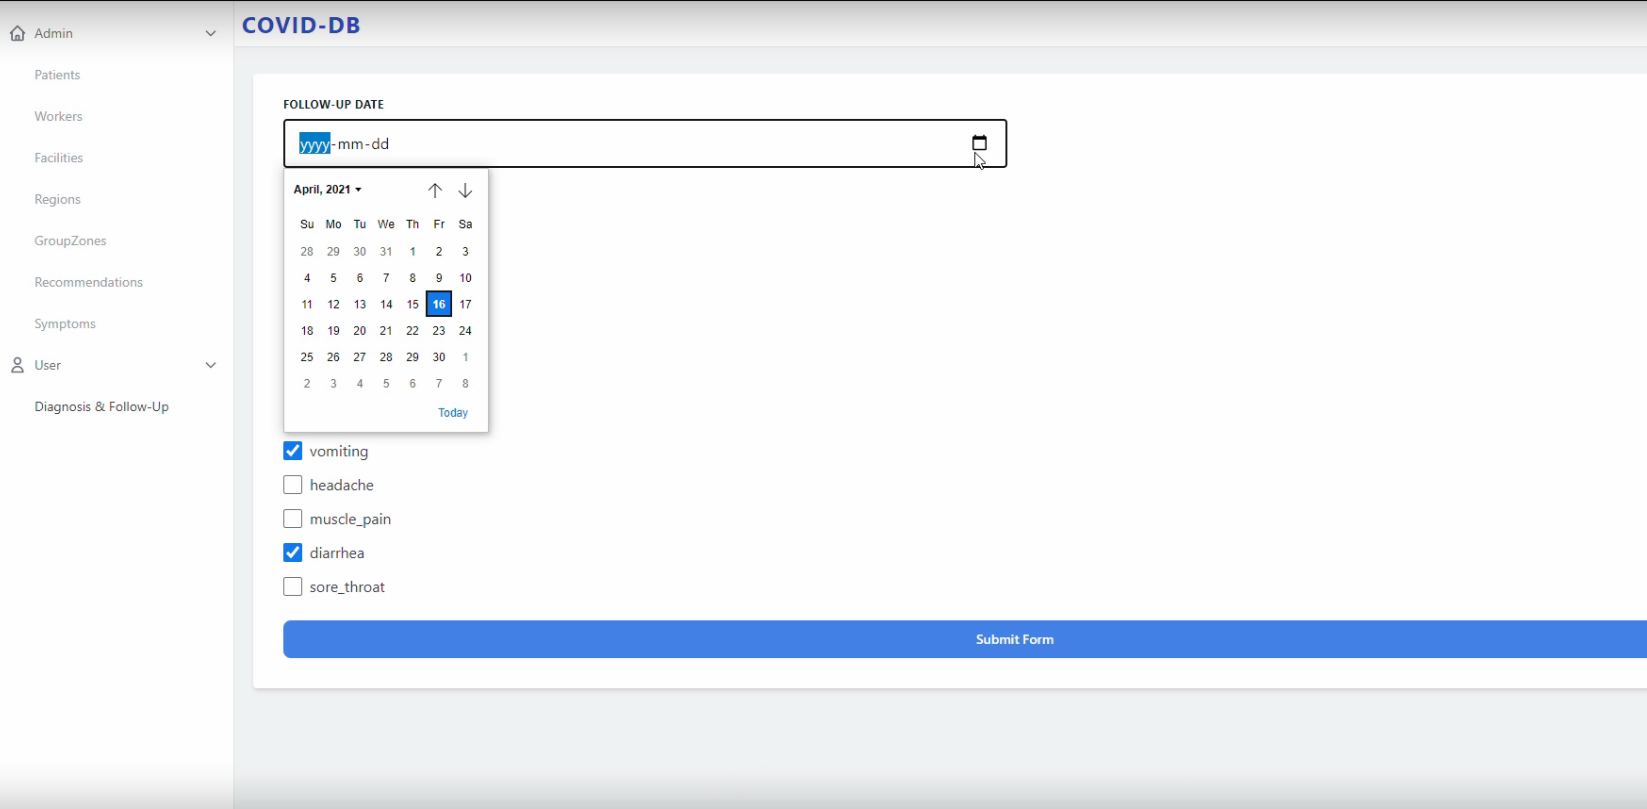
\includegraphics[scale=0.35]{imgs/fillingAForm.PNG}
    \caption{Filling up a form}
\end{figure}


\newpage

%  Q9  % 
\subsection{Symptoms Progress}
Provide a detail progress of all the symptoms for a given person who tested positive on a specific date.
\subsubsection{MySQL}

\begin{minted}{MYSQL}
SELECT (`form_id`),(`patient_id`),(`created_at`),(`symptom`)
FROM followupformsymptompivot 
NATURAL JOIN followupform
NATURAL JOIN symptom 
WHERE patient_id = patient_id AND created_at > start_date
\end{minted}

\subsubsection{PHP}
The implementation in the back-end is written as:
\begin{minted}{php}
<?php
# Q9
public function readAll(Request $request){
return response()->json(DB::select("SELECT (`form_id`),(`patient_id`),(`created_at`),(`symptom`)
FROM followupformsymptompivot 
NATURAL JOIN followupform
NATURAL JOIN symptom 
WHERE patient_id = $request->patient_id AND created_at = $request->start_date"));
}
\end{minted}

\subsubsection{Representative tuples}
An example GET request would be : \\
127.0.0.1:8000/api/form?patient\_id=1\&start\_date='2021-04-17'\\
Which would return something like :
\begin{table}[ht]
\centering
\begin{tabular}{|l|l|l|l|} 
        \hline
        form\_id & patient\_id & created\_at & symptom \\
        \hline 
        4&1& 2021-04-17 10:25:27 & headache\\
        5&1 & 2021-04-18 10:25:27 & throat ache\\
        6&1 & 2021-04-18 21:07:18 & cough\\
        7&1 & 2021-04-18 10:30:00 & cough\\
        8&1 & 2021-04-19 11:00:00 & headache\\
        \hline
\end{tabular}
\caption{Symptom progress representative tuples}
\end{table}
%  Q10  % 
\subsection{Messages during a given time} 
Display all messages generated by the system within a specific period of time.

\subsubsection{MySQL}
\begin{minted}{MYSQL}
SELECT * FROM Messages 
WHERE msg_date > start_date 
AND msg_date < end_date
\end{minted}

\subsubsection{PHP}
The implementation in the back-end is written as:
\begin{minted}{php}
<?php
# Q10
public function readAll(Request $request){
        return response()->json(DB::select("SELECT * FROM messages WHERE msg_date > $request->start_date AND msg_date < $request->end_date"));
}

\end{minted}

\subsubsection{Representative tuples}
An example GET request would be : \\
127.0.0.1:8000/api/messages?start\_date='2021-04-13 23:59:59'\&end\_date=2021-04-17 23:59:59'\\
Which would return something like :
\begin{table}[ht]
    \centering
    \begin{tabular}{|l|l|l|l|l|l|l|} 
        \hline
        msg\_id  & region\_id & msg\_date & alert\_id\ & message & person\_id \\
        \hline 
        45 & NULL & 2021-04-14 15:56:50 & NULL & \multicolumn{1}{m{6cm}|}{Bonsoir Eliott You have recieved a POSITIVE result for you COVID diagnostic.
        Please click here to view the public health recommendations that should be followed \& click here to fill your followup form for the 14 next days} & 6  \\
        46 & NULL & 2021-04-15 15:56:50 & NULL & \multicolumn{1}{m{6cm}|}{Bonsoir Angela. You have recieved a Negative result for you COVID diagnostic.} & 1 \\
       47 & 21 & 2021-04-15 19:06:50 & 4 & \multicolumn{1}{m{6cm}|}{Bonsoir Tyrell. This is an automated message generated at 19:06:50 to warn you that the alert level in you region 5 went from 3 to 4. Click here to read about the new guidelines} & 8  \\
        48 & NULL & 2021-04-15 21:48:23 & NULL & \multicolumn{1}{m{6cm}|}{Bonsoir Tyrell. You have recieved a NEGATIVE result for your COVID diagnostic} & 8  \\
        49 & 5 & 2021-04-17 18:56:50 & 2 & \multicolumn{1}{m{6cm}|}{Bonsoir Eliott. This is an automated message generated at 18:56:50 to warn you that the alert level in you region 5 went from 1 to 2} & 6  \\
        \hline
\end{tabular}
\caption{Messages generated in a given time representative tuples}
\end{table}
\subsubsection{Screenshot in WebApp}    
\begin{figure}[H]
    \centering
    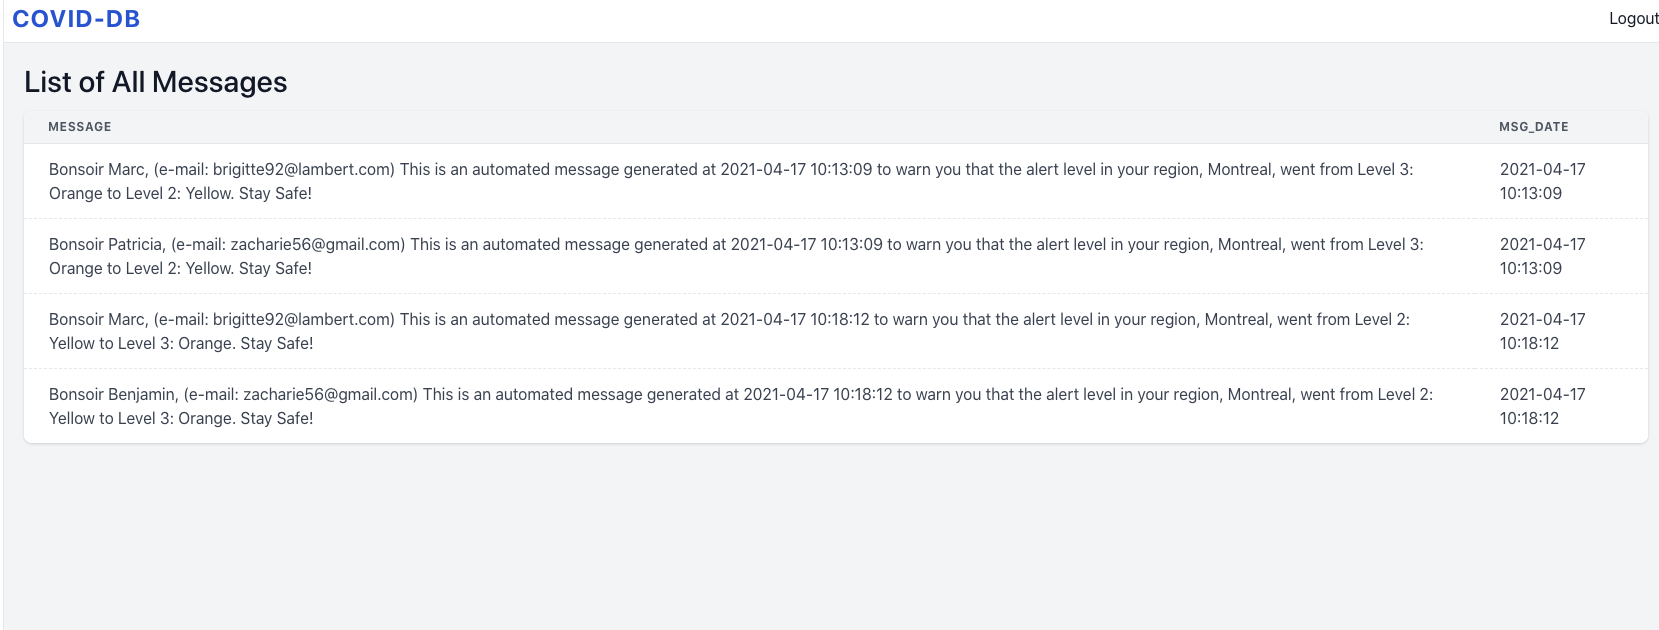
\includegraphics[scale=0.3]{imgs/allmsgs.png}
    \caption{Display all messages generate during in a given time}
\end{figure}

% Q11 %
\subsection{People in an address}
Give a list of all the People in a specific address. For every person, provide
the first name, last name, DOB, medicare card number, telephone number,
citizenship, email address, full mother’s name and full father’s name.
\subsubsection{MySQL}
\begin{minted}{MYSQL}
SELECT ps.first_name, ps.last_name, ps.dob, ps.medicare, ps.phone, ps.citizenship, ps.email,
group_concat(ps2.first_name , ' ', ps2.last_name) as parent_full_name FROM person ps
JOIN carer c ON c.child_id = ps.person_id
JOIN person ps2 ON c.parent_id = ps2.person_id
WHERE ps.address = '3239 Isaac Lake Apt. 198'
GROUP BY medicare;
\end{minted}

\subsubsection{PHP}
\begin{minted}{php}
<?php
public function readAll(Request $request)
{
    $criteria = collect();
    if ($request->filled('address')) {
        $criteria->put("address =  {$request->address}");
    }
    
    $stringQuery = $criteria->count() > 0 ? 'WHERE ' . $criteria->join(',');
    return response()->json(DB::select("SELECT p.patient_id, ps.*
        FROM Patient p
        JOIN Person ps ON p.person_id = ps.person_id $stringQuery"));
}
\end{minted}
\subsubsection{Representative tuples}
Which would return something like :
\begin{table}[ht]
\centering
    \begin{tabular}{|l|l|l|l|l|l|l|} 
        \hline
        first & last & dob & medicare & phone & citizenship & parent full \\
        \hline 
        Christine & Tessier & 1988-08-15 & YNPI68246266 & 18135950684 & US & Nathalie Roy, Jules Langlois\\
        Julie & Titty & 1969-04-20 & ADFY12346214 & 13953393929 & CA & Marcel Bo, Dom Nadeau \\
        Edith & Tardif & 1990-06-29 & GCPI16679278 & (730) 404-1566 & MX & Guillaume\\
        \hline
    \end{tabular}
    \caption{People living in the same address representative tuples.}
    \end{table}
\subsubsection{Screenshot in WebApp}   

\begin{figure}[H]
    \centering
    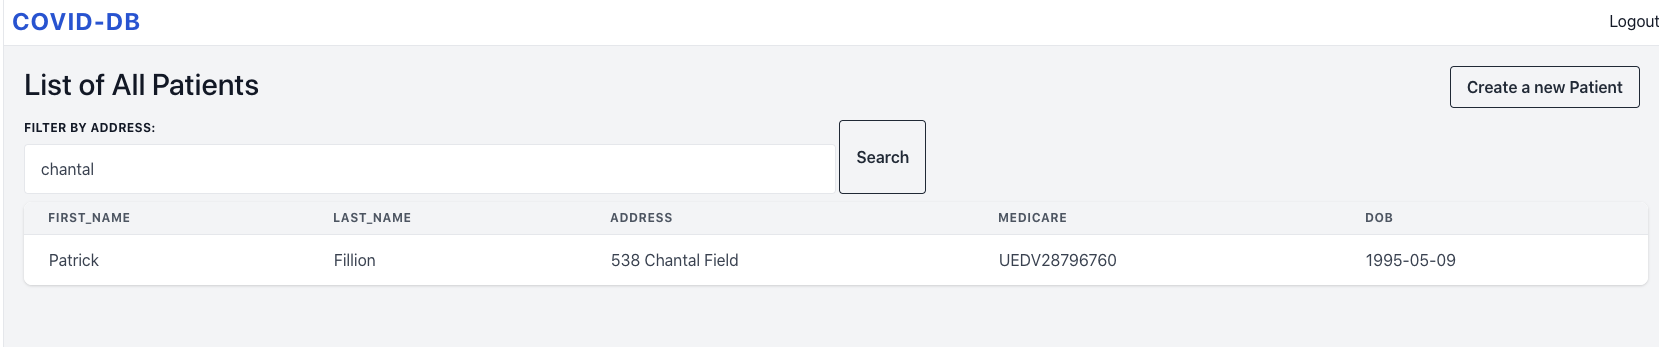
\includegraphics[scale=0.25]{imgs/patientsbyadr.png}
    \caption{Patients in an address}
\end{figure}



\subsection{Details of all facilities}
Give a detail list of all facilities (Address, Number of health workers, accept
walk-in clients or by appointment only, Drive thru capability, etc.).

\subsubsection{MySQL}
\begin{minted}{MYSQL}
SELECT
   phc.`health_center_id`,
   phc.`name`,
   phc.`phone`,
   phc.`address`,
   phc.`type`,
   phc.`method`,
   COUNT(w.health_worker_id) as 'worker_amount',
   if (phc.`drive_thru`, 'Yes','No')
FROM PublicHealthCenter phc
JOIN PublicHealthWorker w ON w.health_center_id = phc.health_center_id
GROUP BY phc.health_center_id

\end{minted}

\subsubsection{PHP}
\begin{minted}{php}
<?php
public function readAll(Request $request)
{
    return response()->json(DB::select("
        SELECT
               phc.`health_center_id`,
               phc.`name`,
               phc.`phone`,
               phc.`address`,
               phc.`type`,
               phc.`method`,
               COUNT(w.health_worker_id) as 'worker_amount',
               if (phc.`drive_thru`, 'Yes','No') as 'drive_thru'
        FROM PublicHealthCenter phc
        JOIN PublicHealthWorker w ON w.health_center_id = phc.health_center_id
        GROUP BY phc.health_center_id"));
}

\end{minted}

\subsubsection{Screenshot in webapp}

\begin{figure}[H]
    \centering
    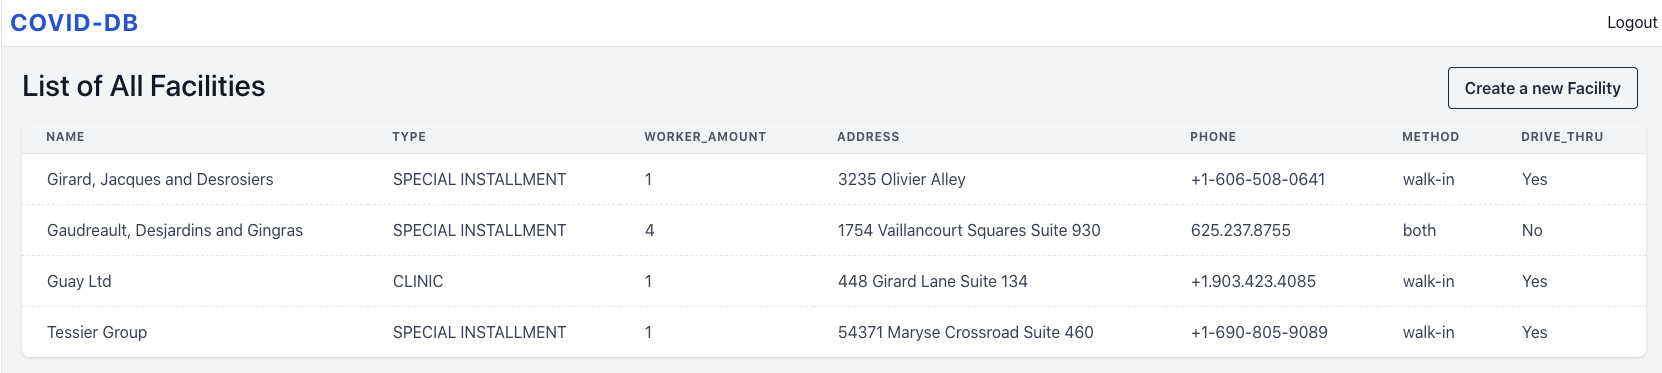
\includegraphics[scale=0.32]{imgs/allfacilities.png}
    \caption{Displaying details of all facilities}
\end{figure}

\subsection{Details of all Regions}
Give a detail list of all Regions (Name, list of all cities within the region,
and a list of all the postal codes within every city). 


\subsubsection{MySQL}
\begin{minted}{MYSQL}
SELECT
    r.region_id,
    r.region_name,
    a.alert_id,
    a.alert_info,
    count(p.person_id) as 'people_amount',
    GROUP_CONCAT(c.city) as 'cities',
    GROUP_CONCAT(pc.postal_code_id) as 'postal_codes'
FROM Region r
JOIN Alert a ON r.alert_id = a.alert_id
JOIN City c ON c.region_id = r.region_id
JOIN PostalCode pc ON pc.city_id = c.city_id
LEFT JOIN Person p ON p.postal_code_id = pc.postal_code_id
GROUP BY r.region_id ORDER BY count(p.person_id) DESC
\end{minted}

\subsubsection{PHP}
\begin{minted}{php}
<?php
public function readAll(Request $request)
{
    return response()->json(DB::select("
        SELECT
            r.region_id,
            r.region_name,
            a.alert_id,
            a.alert_info,
            count(p.person_id) as 'people_amount',
            GROUP_CONCAT(c.city) as 'cities',
            GROUP_CONCAT(pc.postal_code_id) as 'postal_codes'
        FROM Region r
        JOIN Alert a ON r.alert_id = a.alert_id
        JOIN City c ON c.region_id = r.region_id
        JOIN PostalCode pc ON pc.city_id = c.city_id
        LEFT JOIN Person p ON p.postal_code_id = pc.postal_code_id
        GROUP BY r.region_id ORDER BY count(p.person_id) DESC"));
}

\end{minted}

\subsubsection{Screenshot in Webapp}

\begin{figure}[H]
    \centering
    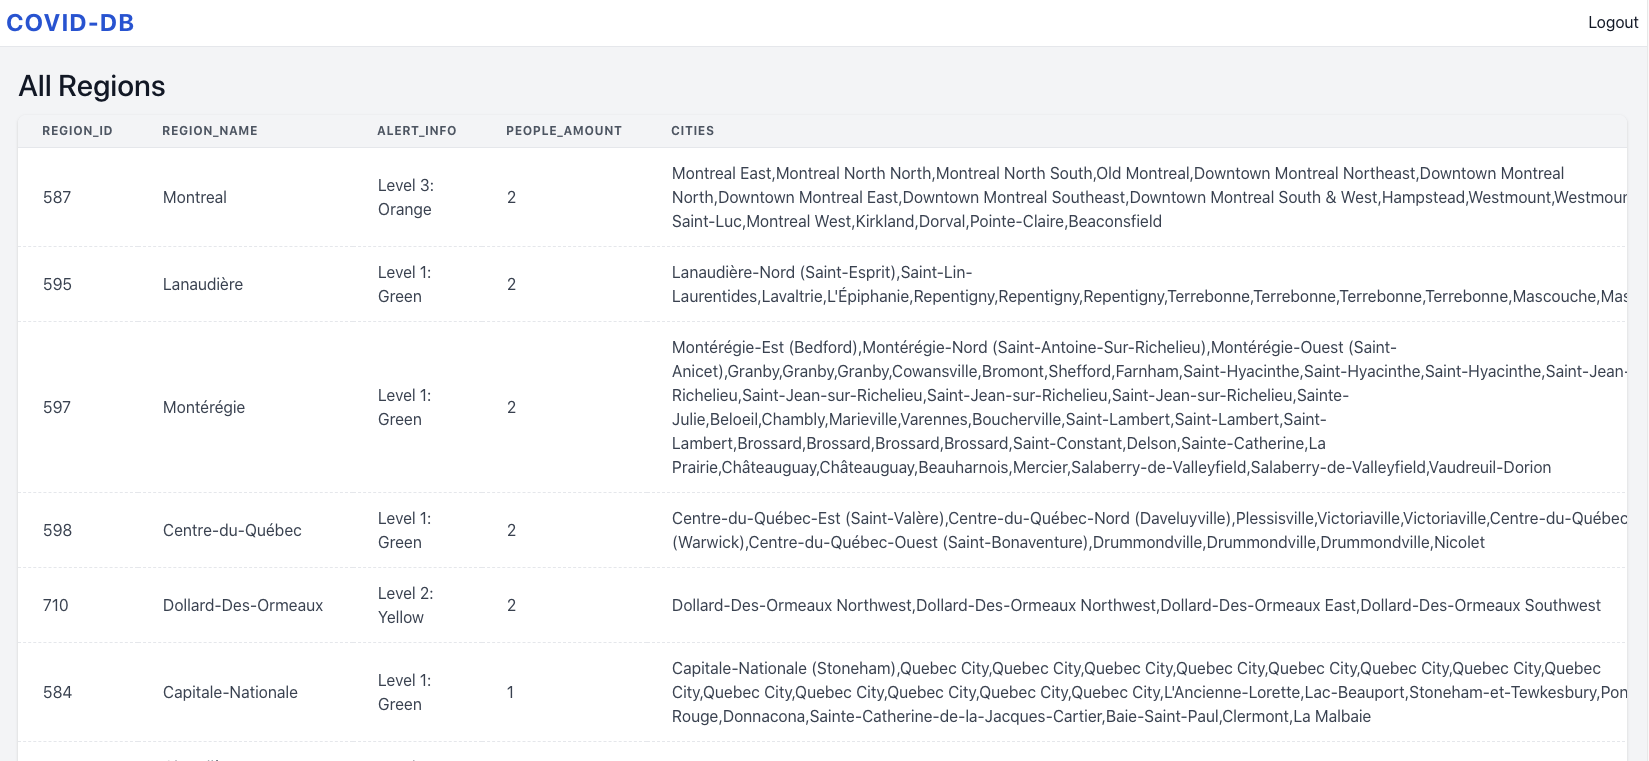
\includegraphics[scale=0.25]{imgs/allregions.png}
    \caption{Displaying details of all regions}
\end{figure}

\subsection{Details of people's test result in a date ordered by result}
Give a List of all people who got the result of the test on a specific date
(Date of the result of the test) grouped by the test result value (First who got
positive result, then who got negative result). The list must include First
Name, Last Name, DOB, Phone Number and email address of the diagnosed
person. 

\subsubsection{MySQL}
\begin{minted}{MYSQL}
SELECT ps.first_name, ps.last_name, ps.dob, ps.phone, ps.email, diagnostic_date, result
FROM diagnostic
NATURAL JOIN patient pt
NATURAL JOIN person ps
WHERE diagnostic_date > '2020-07-01 02:26:24'
ORDER BY result DESC;
\end{minted}

\subsection{List of all workers in a Facility}
Give a list of all workers in a specific facility. 

\subsubsection{MySQL}
\begin{minted}{MYSQL}
SELECT ps.first_name, ps.last_name, health_worker_id FROM publichealthworker
NATURAL JOIN Person ps
WHERE health_center_id = '3'
\end{minted}

\subsection{Workers with COVID at a facility on date and their reach}
Give a list of all public health workers who tested positive on a specific date
in a specific facility. In addition, provide a list of the employees who worked
with the infected health workers for the period of fourteen days prior to the
test. Use the date of the test taken by the infected health worker.

\subsubsection{MySQL}
\begin{minted}{MYSQL}
#6.9(1)
#ALL WORKERS WITH COVID ON THIS DATE AT THIS FACILITY
SELECT * FROM diagnostic
NATURAL JOIN patient pt
NATURAL JOIN person ps
JOIN publichealthworker pw ON pw.person_id = ps.person_id
WHERE result = '1' AND diagnostic_date > 0 AND pw.health_center_id = 2;

#6.9(2)
#RETURN WORKER THAT WORKS AT SAME FACILITY 
SELECT * FROM publichealthworker
WHERE health_center_id = 2
\end{minted}

\subsection{Report for every region}
For all regions, provide a report that include the region name, the number
of people who have positive results, the number of people who have
negative results and a history of alerts within a specific period-of- time. 

\subsubsection{MySQL}
\begin{minted}{MYSQL}
SELECT
    r.region_id,
    r.region_name,
    a.alert_id,
    a.alert_info,
    count(p.person_id) as 'people_amount',
    sum(if(aux.came_positive, 1, 0)) as amount_positive,
    sum(if(aux.came_positive, 0, 1)) as amount_negative,
    GROUP_CONCAT(c.city) as 'cities',
    GROUP_CONCAT(pc.postal_code_id) as 'postal_codes'
FROM Region r
JOIN Alert a ON r.alert_id = a.alert_id
JOIN City c ON c.region_id = r.region_id
JOIN PostalCode pc ON pc.city_id = c.city_id
LEFT JOIN Person p ON p.postal_code_id = pc.postal_code_id
LEFT JOIN (
    SELECT 
       pt.person_id as 'person_id',
       MAX(d.diagnostic_date) 'last_diagnostic_date',
       MAX(d.result) as 'came_positive'
    FROM Patient pt
      JOIN Diagnostic d ON pt.patient_id = d.patient_id
      GROUP BY pt.person_id
      ORDER BY MAX(d.diagnostic_date) 
) as aux ON aux.person_id = p.person_id
GROUP BY r.region_id ORDER BY count(p.person_id) DESC;
\end{minted}

\newpage
\section{User Interface}

\begin{figure}[H]
    \centering
    \includegraphics[scale=0.25]{imgs/UserInterface.png}
    \caption{Landing Page of the User}
\end{figure}

\subsection{Linked Resources}

\textbf{GitHub URL}: https://github.com/wdlnph/coviddb

\textbf{Live Site URL}: https://ydc353.encs.concordia.ca/coviddb/portal

\subsection{Backend Component: Laravel}

The COVID-DB Application was built by our team using the Laravel PHP Framework, built by Taylor Otwell in June 2011. Not only does it help with proper session handling, password encryption and security layers for our service, but it also provides an simple organized MVC directory layout where we can properly separate our back-end component from the front end one. This allowed for the team to be highly effective during implementation, as the Controllers would be able to be implemented concurrently to the UI Layouts to be built

To accommodate with the requirements provided to us, some compromises were made to omit the use of some features in Laravel.

\textbf{Fluent Language}

Rather than using the fluent language, we have opted to write direct SQL into our service, allowing for the marker to properly verify that the queries have been implemented

\textbf{Migrations}

A new file create\_tables.sql was created in /database/sql folder to provide all the Relations that were created throughout this project, rather than the turnkey migration solution commonly performed in Laravel.

\textbf{Seeding}

Factory files were also omitted. Instead, we have provided the files insert\_statements.sql, insert\_regions.sql and triggers.sql to ensure the database is populated in the way it should match results found in this report.

\subsection{Frontend Component: ReactJS}

For a highly intuitive interface, we have opted to make use of the ReactJS framework for our front end. React allows us to easily re-use components throughout multiple entities, and provide a simple way to validate forms and communicate with the backend component. The axios package was used to communicate with the API, and the Formik plugin is used for validation with Yup. 

In addition, we have decided to use Tailwind CSS to design our components, all of which is compiled using the Webpack wrapper provided by Laravel Mix.


\subsection{Authentication}
\\
The user is able to log in using his medicare card and password, which is its date of birth, in YYYYMMDD format. A register functionality would also be provided, as well as a forgot password and remember me checkbox. These, however, do not enter into the scope of this project.

\begin{figure}[H]
    \centering
    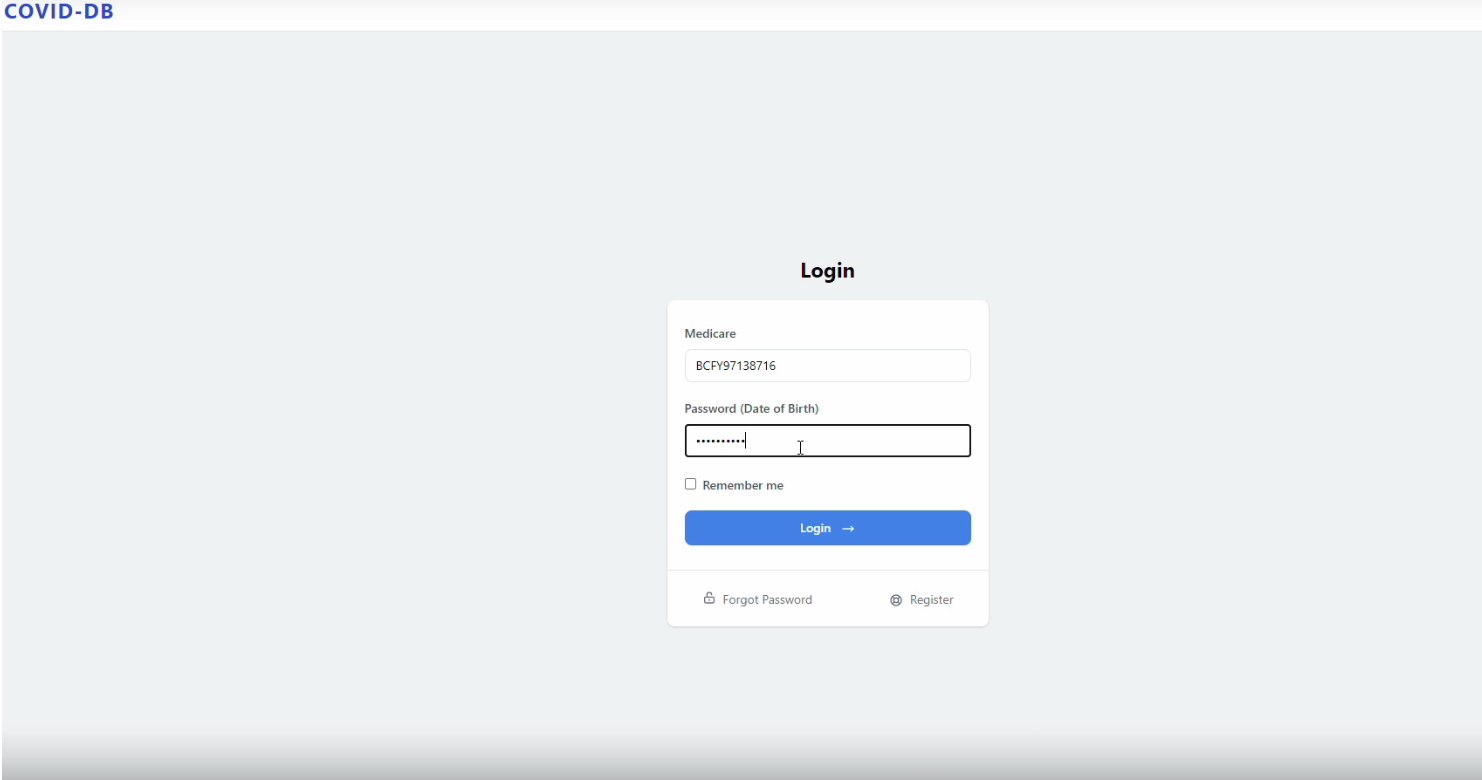
\includegraphics[scale=0.35]{imgs/loginScreen.PNG}
    \caption{Home Page allows you to login with your medicare and dob}
\end{figure}

\subsection{CRUD Table}

A table was designed to display information coming from any `readAll` functions. These rows can be clicked to further go into the Edit Entity page in order to update the selected row. Depending on the page, some filters may be provided at the top of the page.

\begin{figure}[H]
    \centering
    \includegraphics[scale=0.25]{imgs/CRUDTable.png}
    \caption{List of all workers in a table}
\end{figure}

\subsection{Create/Update Entity}

Each entity provides its own schema that can be validated using the combination of the Yup and Formik plugins. Validation prevents for erroneous data from reaching the database, as it may not result into the right constraints being respected. This only serves as a first layer protection, since the Database and the API itself provide their own validation rules as well.

The form has been made to accommodate both the creation and update of a record. a delete option is also provided at the bottom in order to delete the entity if needed.

\begin{figure}[H]
    \centering
    \includegraphics[scale=0.25]{imgs/EditCreateUser.png}
    \caption{This edit page provides feedback on what has not been filled out by the user}
\end{figure}

\subsection{Toast notification}

The Toast plugin allows us to provide to the user any information that is pertaining to him if they come to be.


\begin{figure}[H]
    \centering
    \includegraphics[scale=0.25]{imgs/Toast.png}
    \caption{A toast notification}
\end{figure}


\subsection{Region Update}

We have made the assumption that a Region cannot be deleted. Therefore, this leaves only the ability for us to update the alert level. We have therefore taken the liberty to provide a more in depth view that explains some restrictions related to the alert in place. This information can be toggled, however the information is hard coded into the application rather than in the database.

\begin{figure}[H]
    \centering
    \includegraphics[scale=0.25]{imgs/EditRegion.png}
    \caption{Edit Region Form}
\end{figure}


\section{Bonus: Additional feature}
\subsection{Twilio SMS API Integration}

Using the Twilio Messaging API, We can set up a cronjob which fetches any messages that have yet to be sent

\subsubsection{MySQL Query}
\begin{minted}{MYSQL}
SELECT
    m.msg_id,
    m.message,
    p.phone
FROM Messages m
JOIN Person p ON p.person_id = m.person_id
WHERE is_sent = 0
\end{minted}

\subsubsection{PHP Command}

\begin{minted}{php}
<?php
public function handle()
{
    // Fetch all unsent notifications
    $results = DB::select("SELECT
        m.msg_id,
        m.message,
        p.phone
    FROM Messages m
    JOIN Person p ON p.person_id = m.person_id
                WHERE is_sent = 0");

    $updateMsgs = collect();
    foreach ($results as $result) {
        // Only send to the configured phones
        if (in_array($result->phone, explode(',', env('TWILIO_ALLOWED_PHONES')))) {
            // Send it to the user here
            $this->line("Sending to {$result->phone}");
            $client = new Client(
                env('TWILIO_ACCOUNT_SID'),
                env('TWILIO_AUTH_TOKEN')
            );
            $client->messages->create($result->phone, [
                "body" => $result->message,
                "from" => env("TWILIO_PHONE_NUMBER"),
            ]);
        }
        $updateMsgs->add($result->msg_id);
    }
    $stringUpdate = $updateMsgs->join(',');
    DB::update("UPDATE Messages SET is_sent=1 WHERE msg_id IN ($stringUpdate)");

    $this->line("Successfully Sent " . $updateMsgs->count() . " messages.");
    return 0;
}
\end{minted}

\subsubsection{Twilio Configuration}

A phone number was purchased from the Twilio Console, allowing for the delivery of messages to the Canadian carrier network

\begin{figure}[h]
    \centering
    \includegraphics[scale=0.50]{imgs/PhoneConfiguration.png}
    \caption{Phone Configuration in the Twilio Console}
\end{figure}

\begin{figure}[h]
    \centering
    \includegraphics[scale=0.75]{imgs/EnvironmentVariables.png}
    \caption{Our webapp sends text messages using the Twilio SMS API}
\end{figure}
\subsubsection{Cron Execution}

The cron runs every minute to verify any unsent messages created from the MySQL trigger, and proceeds to update the messages 'is\_sent' value, and sending to the appropriate avenues

\begin{figure}[h]
    \centering
    \includegraphics[scale=0.75]{imgs/CronExecution.png}
    \caption{The command executes to process any unsent messages in the database}
\end{figure}

\begin{figure}[h]
    \centering
    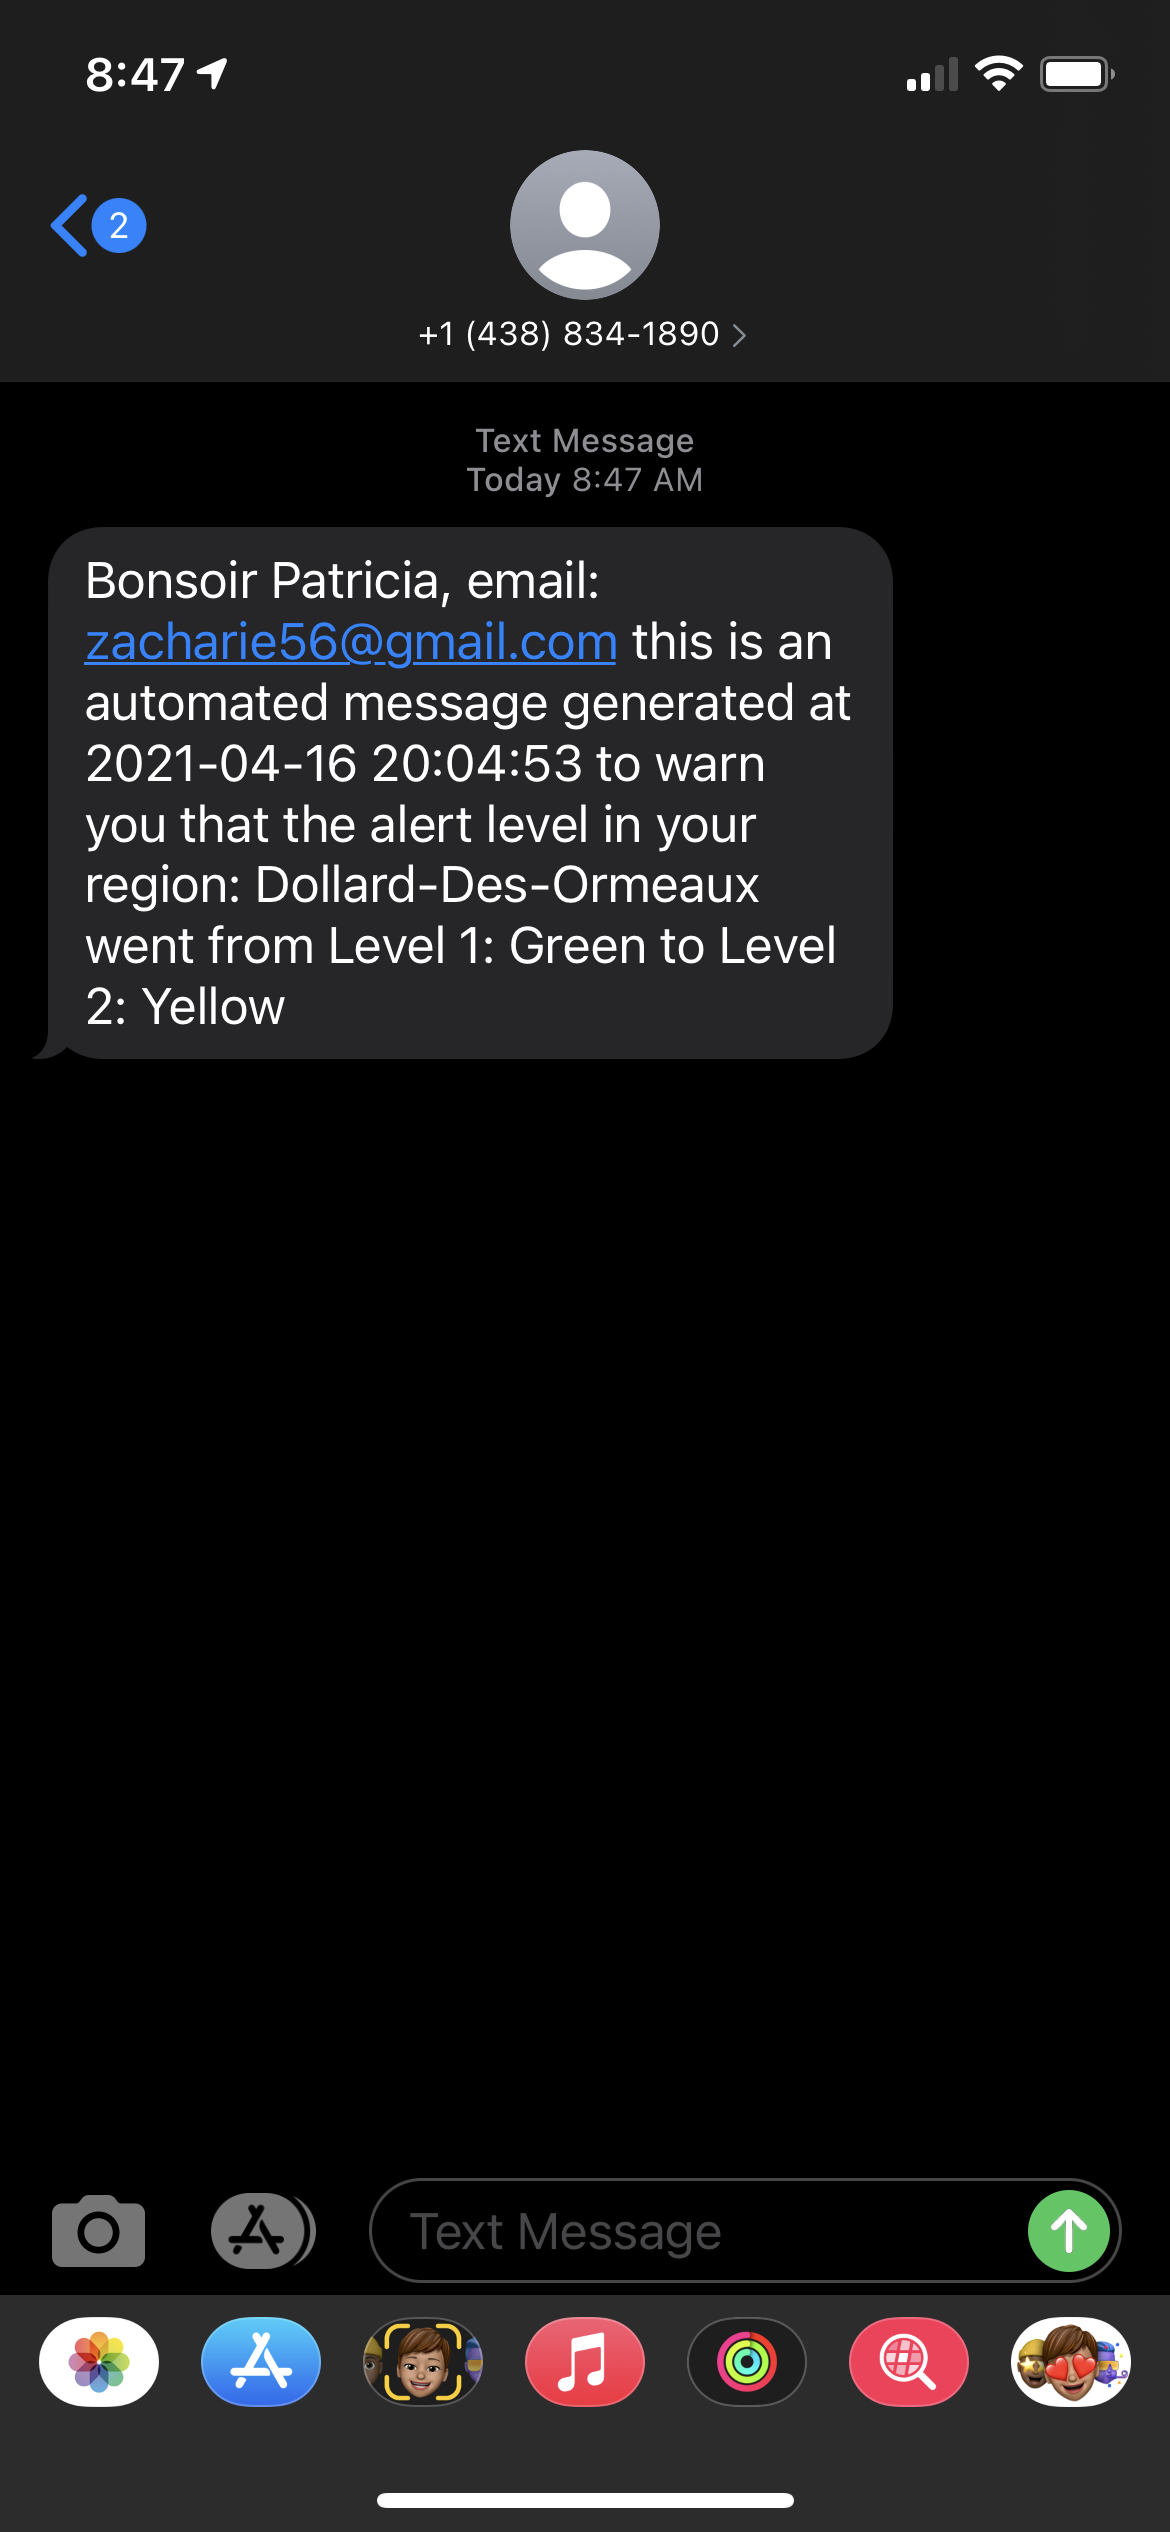
\includegraphics[scale=0.15]{imgs/sms.png}
    \caption{Our webapp sends text messages using the Twilio SMS API}
\end{figure}
\clearpage
\section{Contribution \& Separation of work}
\textbf{Antoine Assal - 40022745}
\begin{itemize}
    \item E/R Diagram
    \item Relational Schema 
    \item Normalization
    \item SQL Queries
    \item PHP controllers
    \item Report
\end{itemize}
\textbf{Benjamin Lofo Follo  - 40008156}
\begin{itemize}
    \item Server Installation
    \item User Interface Components
    \item PHP API Integration
    \item Twilio Integration 
    \item Report section 8
\end{itemize}
\textbf{Rami Bou Abboud  - 40043011}
\begin{itemize}
    \item E/R Diagram
    \item Relational Schema
    \item SQL Table creation
    \item Constraints and triggers
    \item PHP API Integration
\end{itemize}
\textbf{Ribelle El Ayoubi  - 29276726}
\begin{itemize}
    \item User Interface Components
    \item Forms for creation/edits
    \item User Interface Validation
    \item Report section 7 
    \item References
\end{itemize}

\section{References}
\begin{itemize}
    \item \href{https://laravel.com/docs/8.x}{\textcolor{blue}{Laravel}}
    \item \href{https://reactjs.org/docs/getting-started.html}{\textcolor{blue}{ReactJS}}
    \item \href{https://tailwindcss.com/docs}{\textcolor{blue}{TailwindCSS}}
    \item \href{https://tailwindui.com/}{\textcolor{blue}{Tailwind CSS components}}
    \item \href{https://opentextbc.ca/dbdesign01/chapter/chapter-12-normalization/}{\textcolor{blue}{Normalization}}
    \item \href{https://www.w3schools.com/sql/}{\textcolor{blue}{SQL queries}}
    \item \href{https://www.twilio.com/docs/sms}{\textcolor{blue}{Twilio SMS API}}
\end{itemize}




\end{document}
